\section{问题二:玻璃文物分类、亚类划分及可靠性分析}

本部分的目标是根据文物的化学成分,建立高钾玻璃与铅钡玻璃的分类规律,并对两类玻璃进行内部亚类的划分,最后对所得结论的可靠性进行系统性分析。其框架如图\ref{fig:problem2_framework}所示。

\begin{figure}[H]
    \centering
    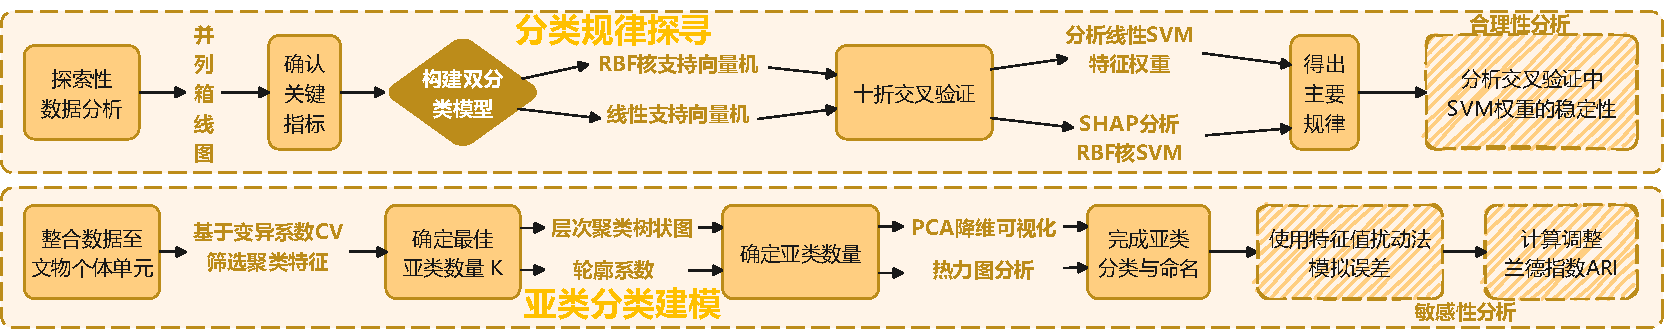
\includegraphics[width=\textwidth]{figs/4问题二/第二问框架.pdf}
    \caption{问题二框架}
    \label{fig:problem2_framework}
\end{figure}

\subsection{高钾玻璃与铅钡玻璃的分类规律}

在构建分类模型之前,首先需要通过探索性数据分析对不同类别的数据在数值特征上的分布差异建立直观认知,这为后续的建模方向和假设形成提供依据。我们采用并列箱线图来直观对比高钾玻璃与铅钡玻璃在全部十四种化学成分含量上的分布差异。

\begin{figure}[H]
    \centering
    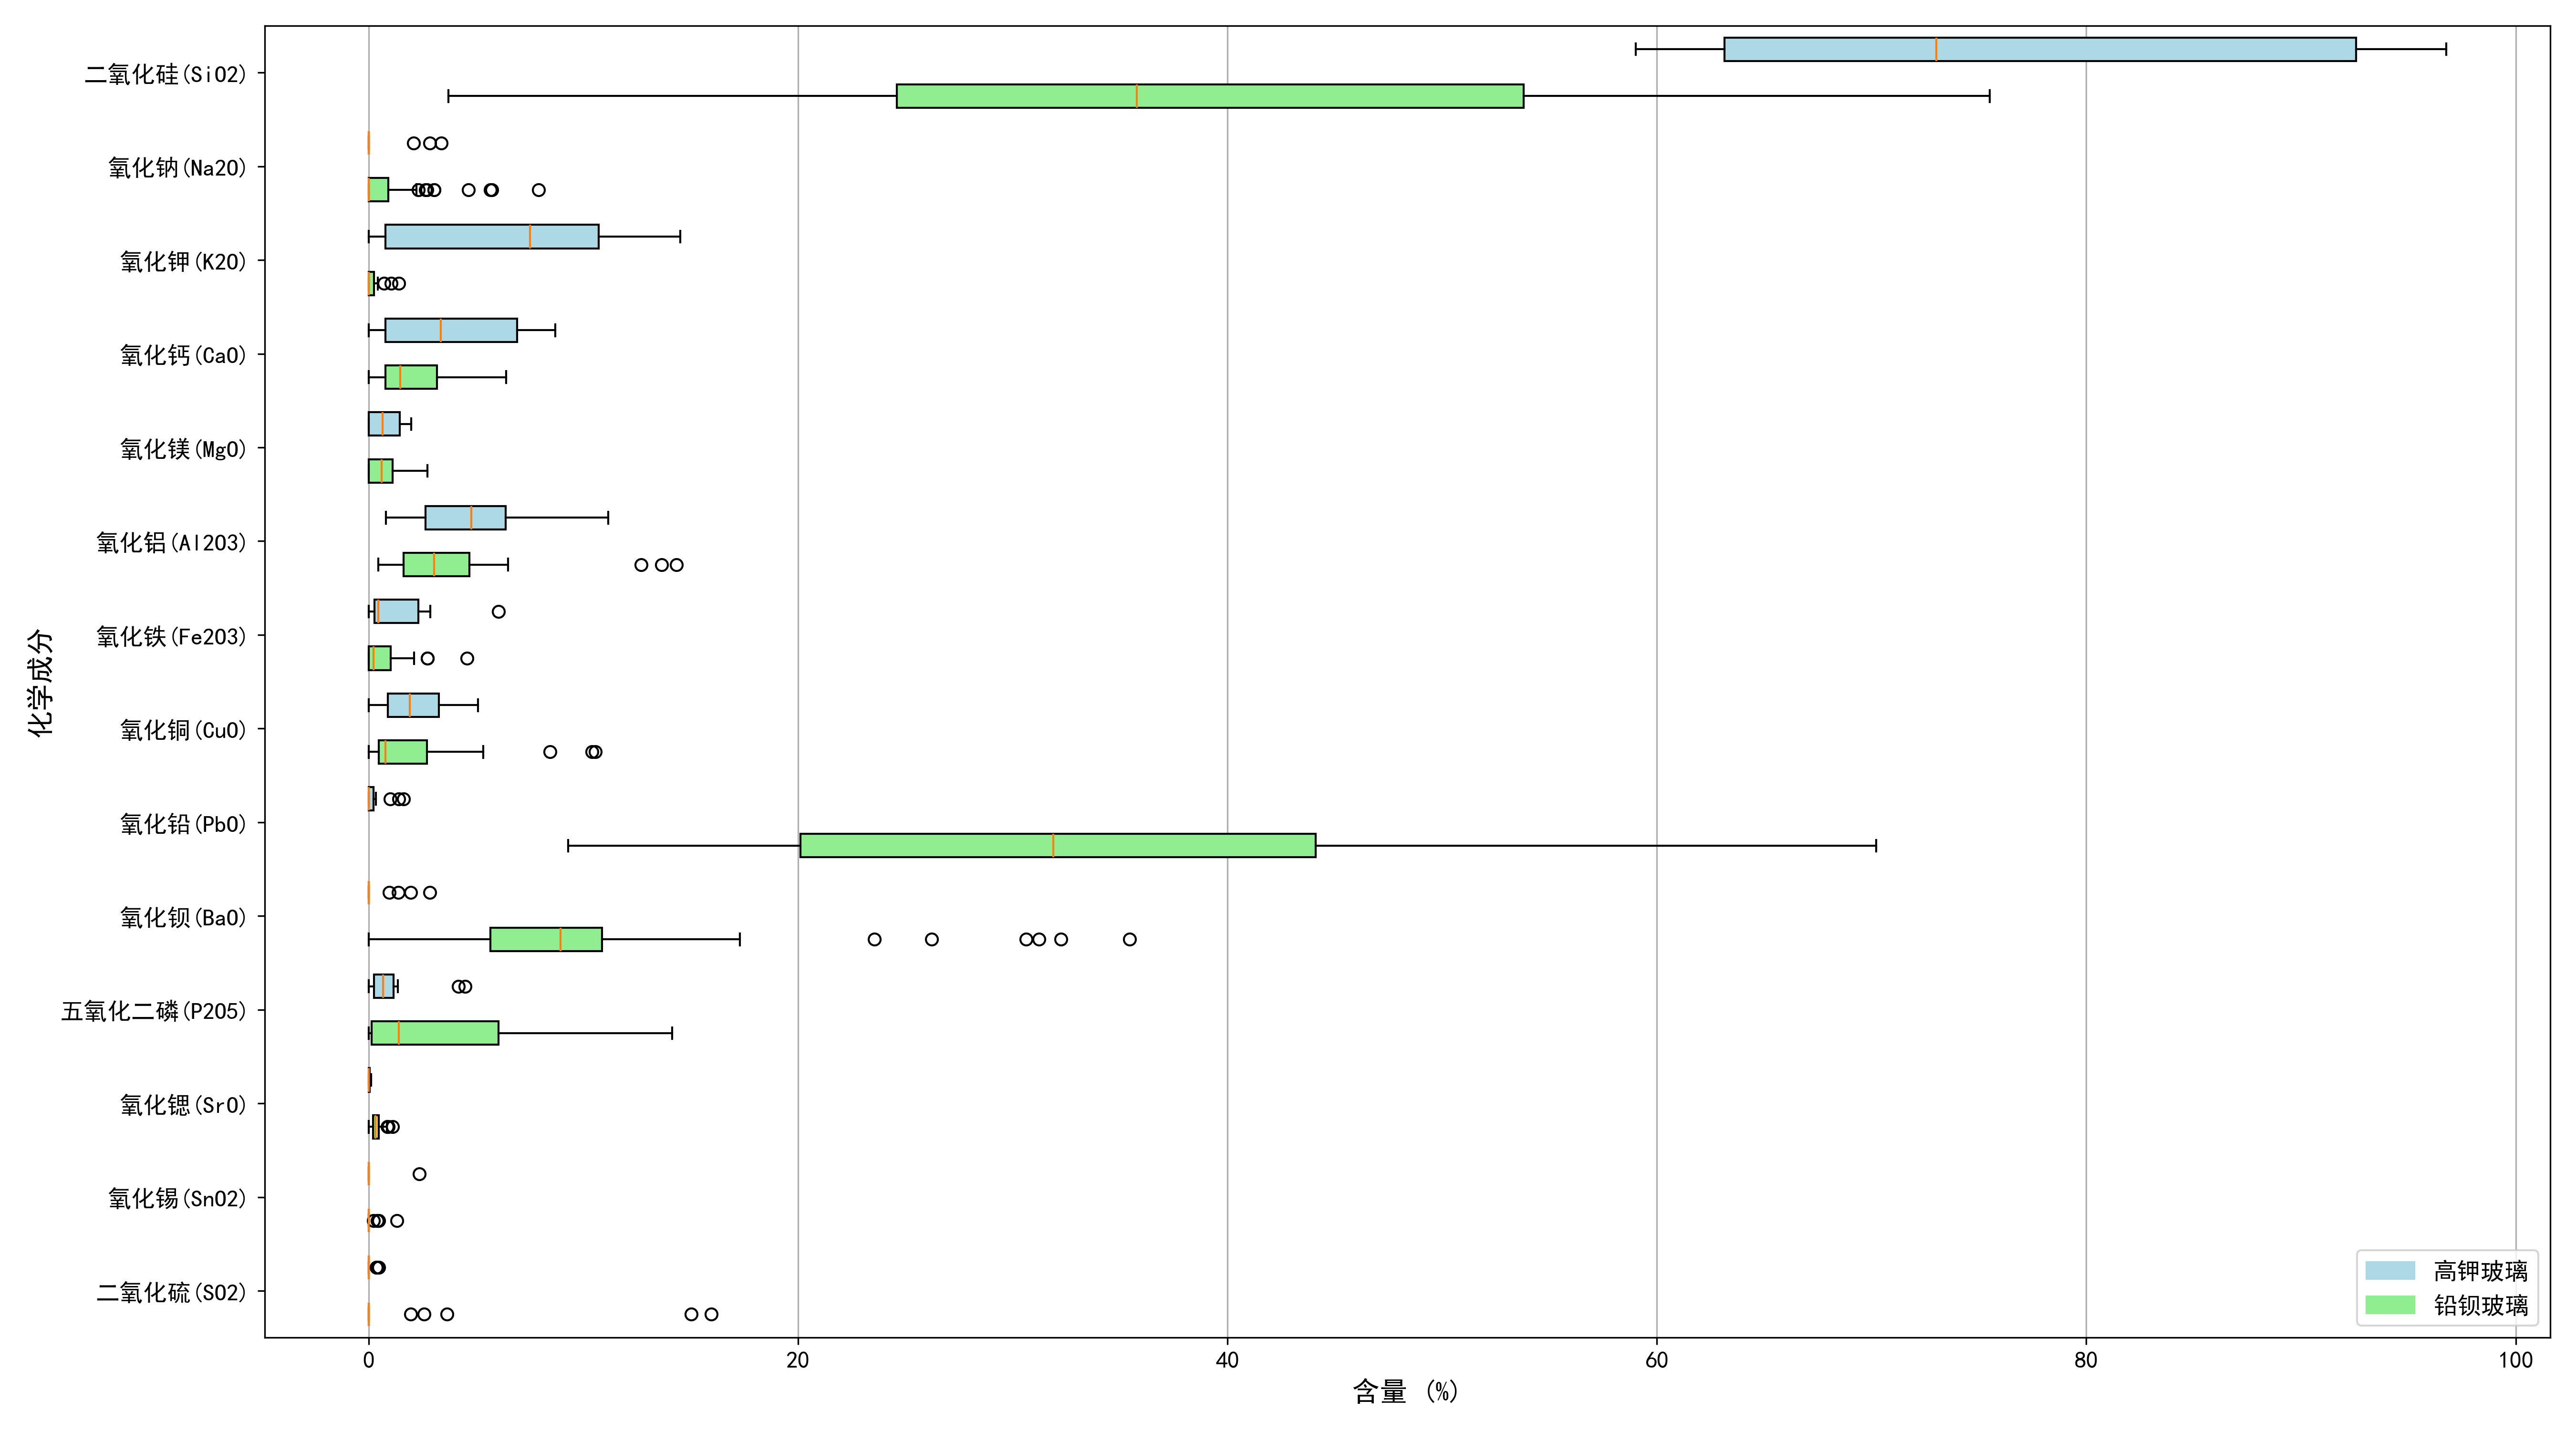
\includegraphics[width=\textwidth]{figs/4问题二/EDA_并列箱线图.png}
    \caption{高钾玻璃与铅钡玻璃化学成分含量分布对比}
    \label{fig:eda_boxplot}
\end{figure}

如图\ref{fig:eda_boxplot}所示,图中纵轴为化学成分,横轴为含量百分比。对于每一种成分,均并排展示了两个箱体,分别代表高钾玻璃和铅钡玻璃的含量分布。由图可知,在氧化铅$PbO$与氧化钡$BaO$两种成分上,铅钡玻璃的含量分布远高于高钾玻璃,而在氧化钾$K_2O$上则呈现相反的模式。两个类别在这些关键成分上的分布区间几乎没有重叠,由此形成核心假设,即$PbO$、$BaO$与$K_2O$是区分两类玻璃的关键指标。

基于前述探索性分析形成的假设,即特定化学成分含量可有效区分玻璃类型,我们构建监督学习分类模型以对该规律进行量化验证。为兼顾模型的解释性与对数据复杂关系的拟合能力,我们分别建立了线性支持向量机与使用径向基函数核的非线性支持向量机模型。

线性支持向量机的基本原理是在一个多维特征空间中,寻找一个最优的分类超平面。该超平面由法向量$\boldsymbol{w}$和位移$b$定义,其数学形式为$\boldsymbol{w}^T\boldsymbol{x} + b = 0$。最优化的目标是不仅能将两类样本分开,同时能最大化距离超平面最近的样本,即支持向量,到超平面的间隔。在允许部分样本被错误分类以增强模型泛化能力的情况下,该问题可表述为一个软间隔优化问题,其目标函数如下
\begin{equation}
    \min_{\boldsymbol{w}, b, \boldsymbol{\xi}} \frac{1}{2} ||\boldsymbol{w}||^2 + C \sum_{i=1}^{m} \xi_i
\end{equation}
式中$C$为正则化系数,用于平衡间隔最大化与分类误差,$\xi_i$是松弛变量,允许样本点在一定程度上偏离其正确的分类边界。

当化学成分与玻璃类型的关系无法通过线性边界有效分离时,需要引入非线性模型。非线性支持向量机通过核技巧将原始特征空间映射到一个更高维度的空间,并在新空间中构造线性超平面。我们选用径向基函数核,即高斯核,作为映射函数,其定义为
\begin{equation}
    K(\boldsymbol{x}_i, \boldsymbol{x}_j) = \exp(-\gamma ||\boldsymbol{x}_i - \boldsymbol{x}_j||^2)
\end{equation}
其中$\gamma$是核函数的一个参数,它决定了单个训练样本影响范围的大小。通过使用该核函数,模型能够在原始空间中形成复杂的非线性决策边界。

为获得稳健的模型性能评估,避免因单次数据划分带来的偶然性,我们采用十折交叉验证方法。该方法将数据集随机分为十个互斥的子集,轮流使用其中九个作为训练集,一个作为测试集,最终以十次测试结果的平均值作为模型的性能度量。评估结果显示,线性支持向量机模型的平均分类准确率为95.71\%,而使用径向基函数核的非线性支持向量机模型平均分类准确率达到97.41\%。两个模型均表现出较高的分类能力。

为解释模型的分类机理,我们首先分析了线性支持向量机学习到的特征权重。

\begin{figure}[H]
    \centering
    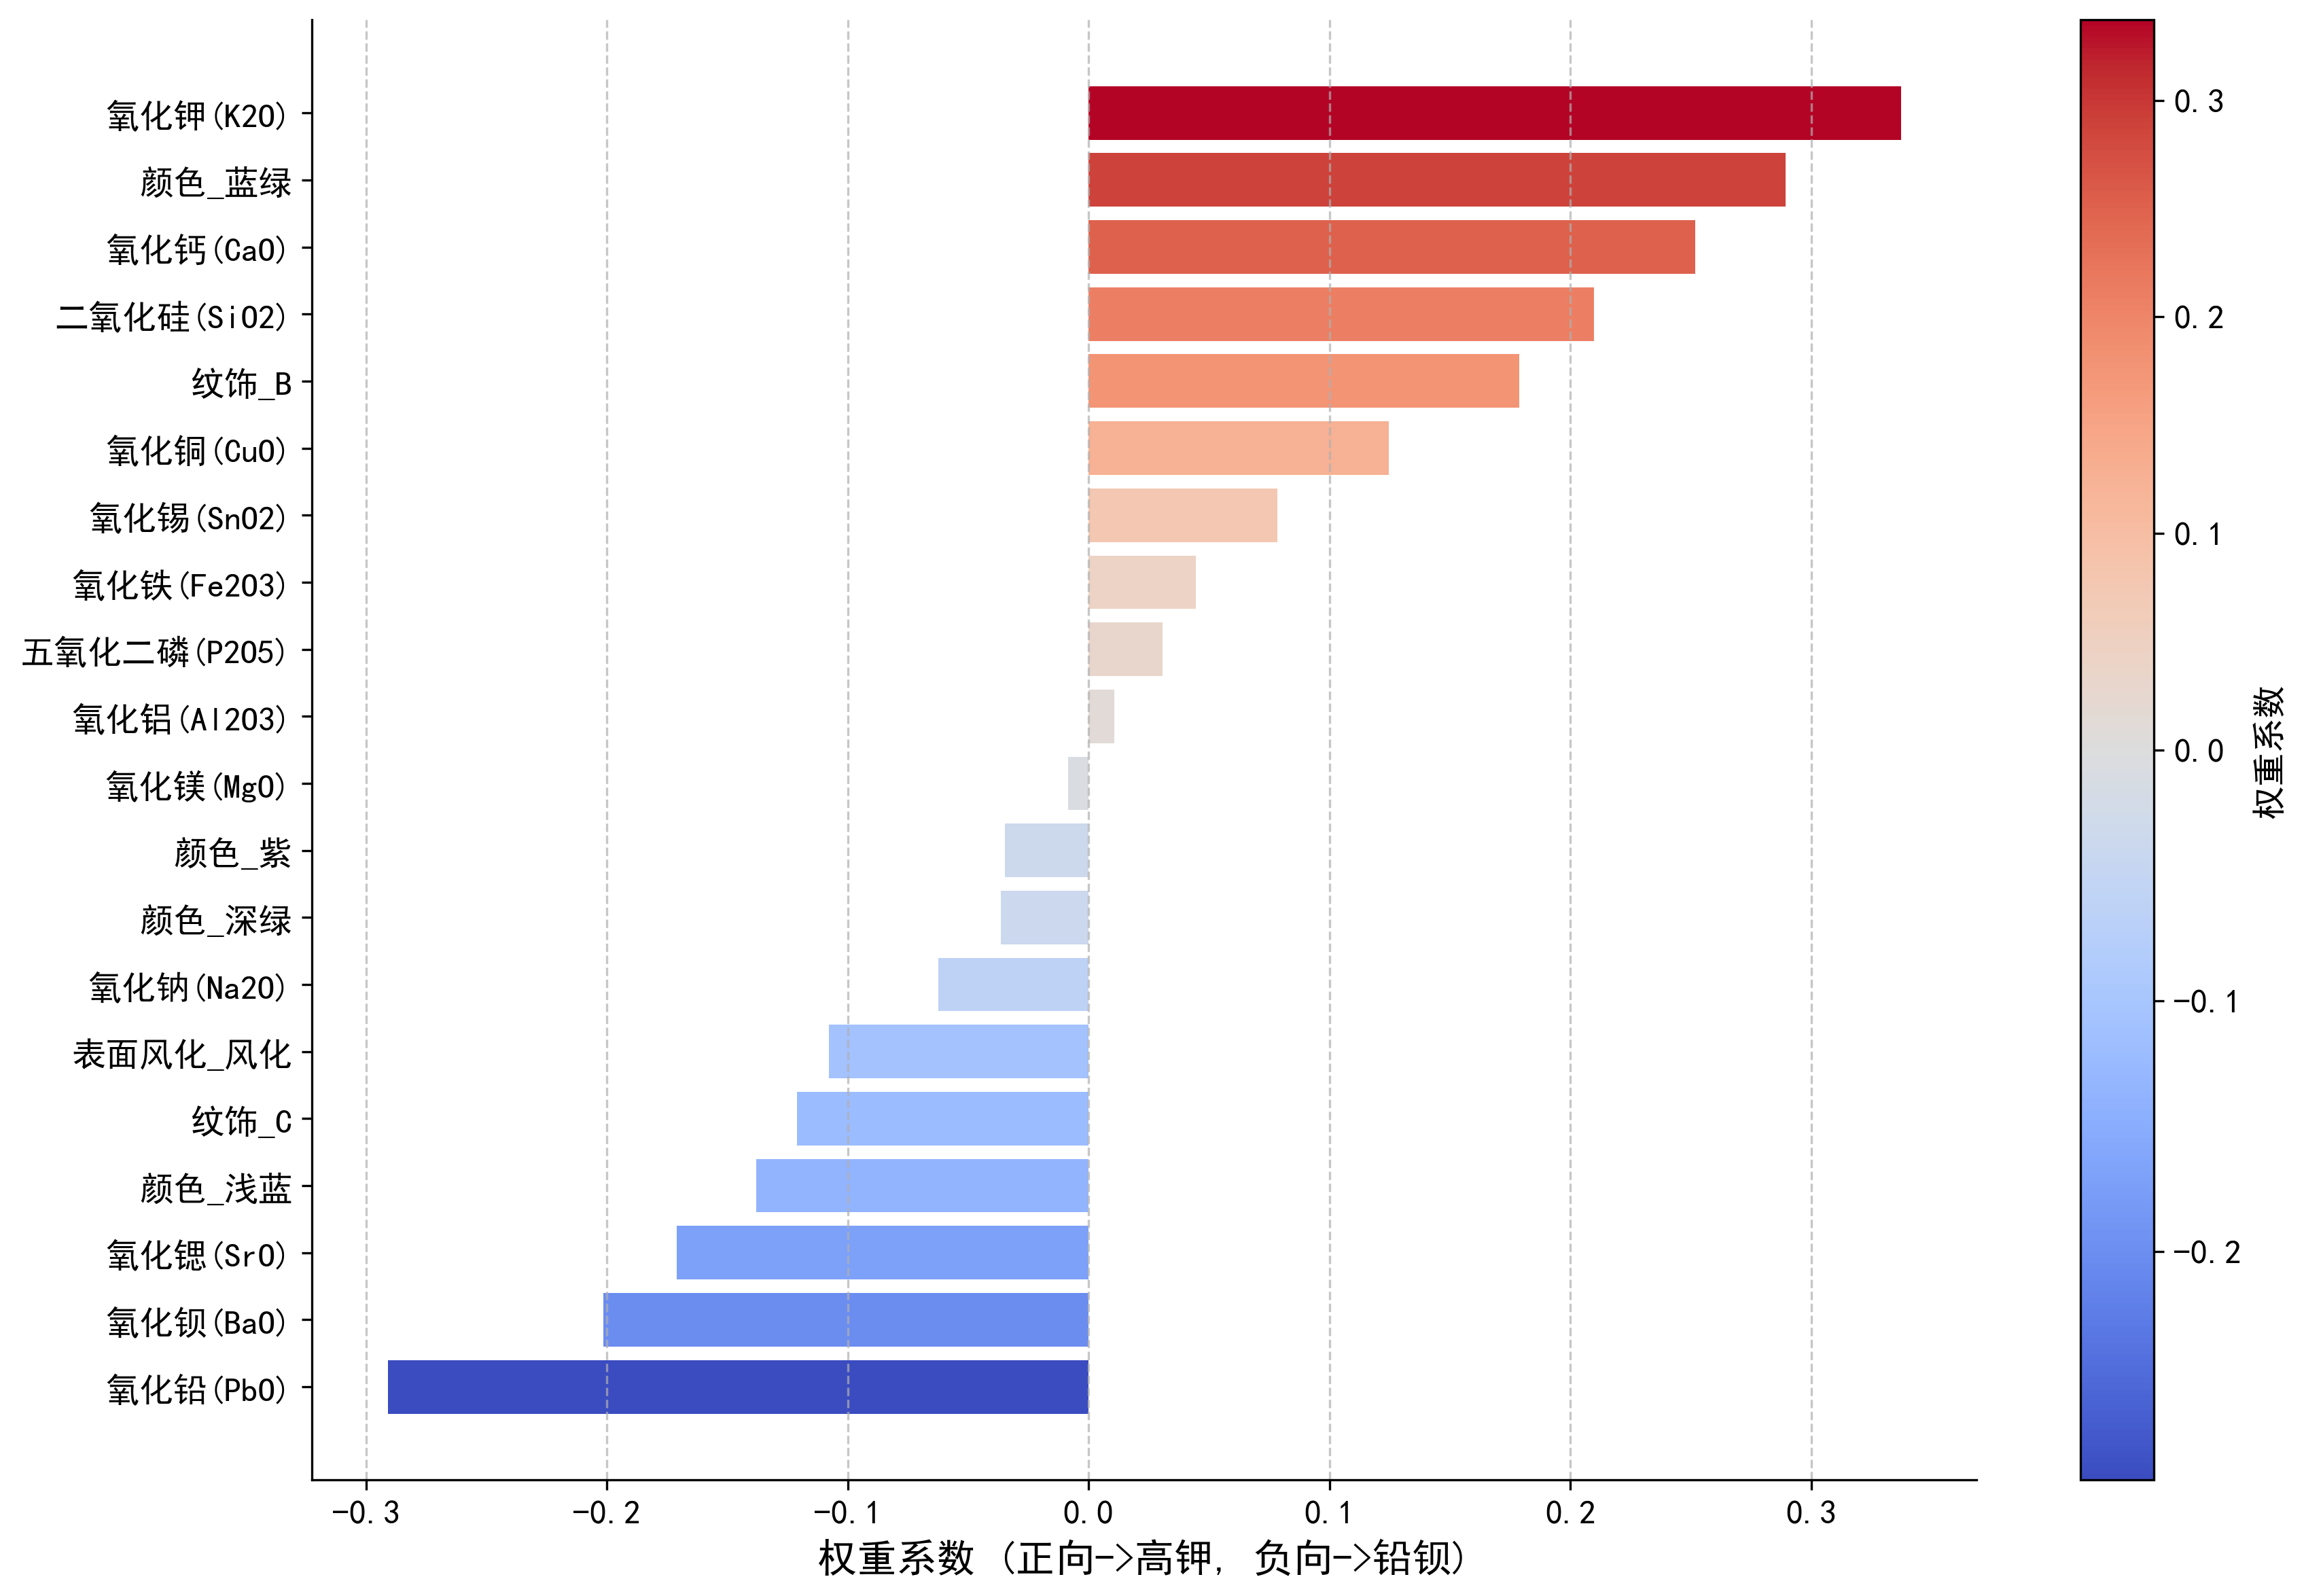
\includegraphics[width=\textwidth]{figs/4问题二/线性SVM特征权重_渐变色.png}
    \caption{线性支持向量机模型学习的特征权重}
    \label{fig:svm_weights}
\end{figure}

图\ref{fig:svm_weights}展示了各化学成分的权重系数值,其中正向权重将预测推向高钾玻璃,负向权重则推向铅钡玻璃。图中可见,氧化钾$K_2O$与二氧化硅$SiO_2$获得了最大的正权重,而氧化铅$PbO$与氧化钡$BaO$获得了最大的负权重,这与探索性分析的发现一致。

对于性能更高但解释性较弱的非线性模型,我们采用SHAP,即SHapley Additive exPlanations框架进行分析。该方法基于合作博弈论,能够将模型的预测结果公平地归因到每个输入特征上。

\begin{figure}[H]
    \centering
    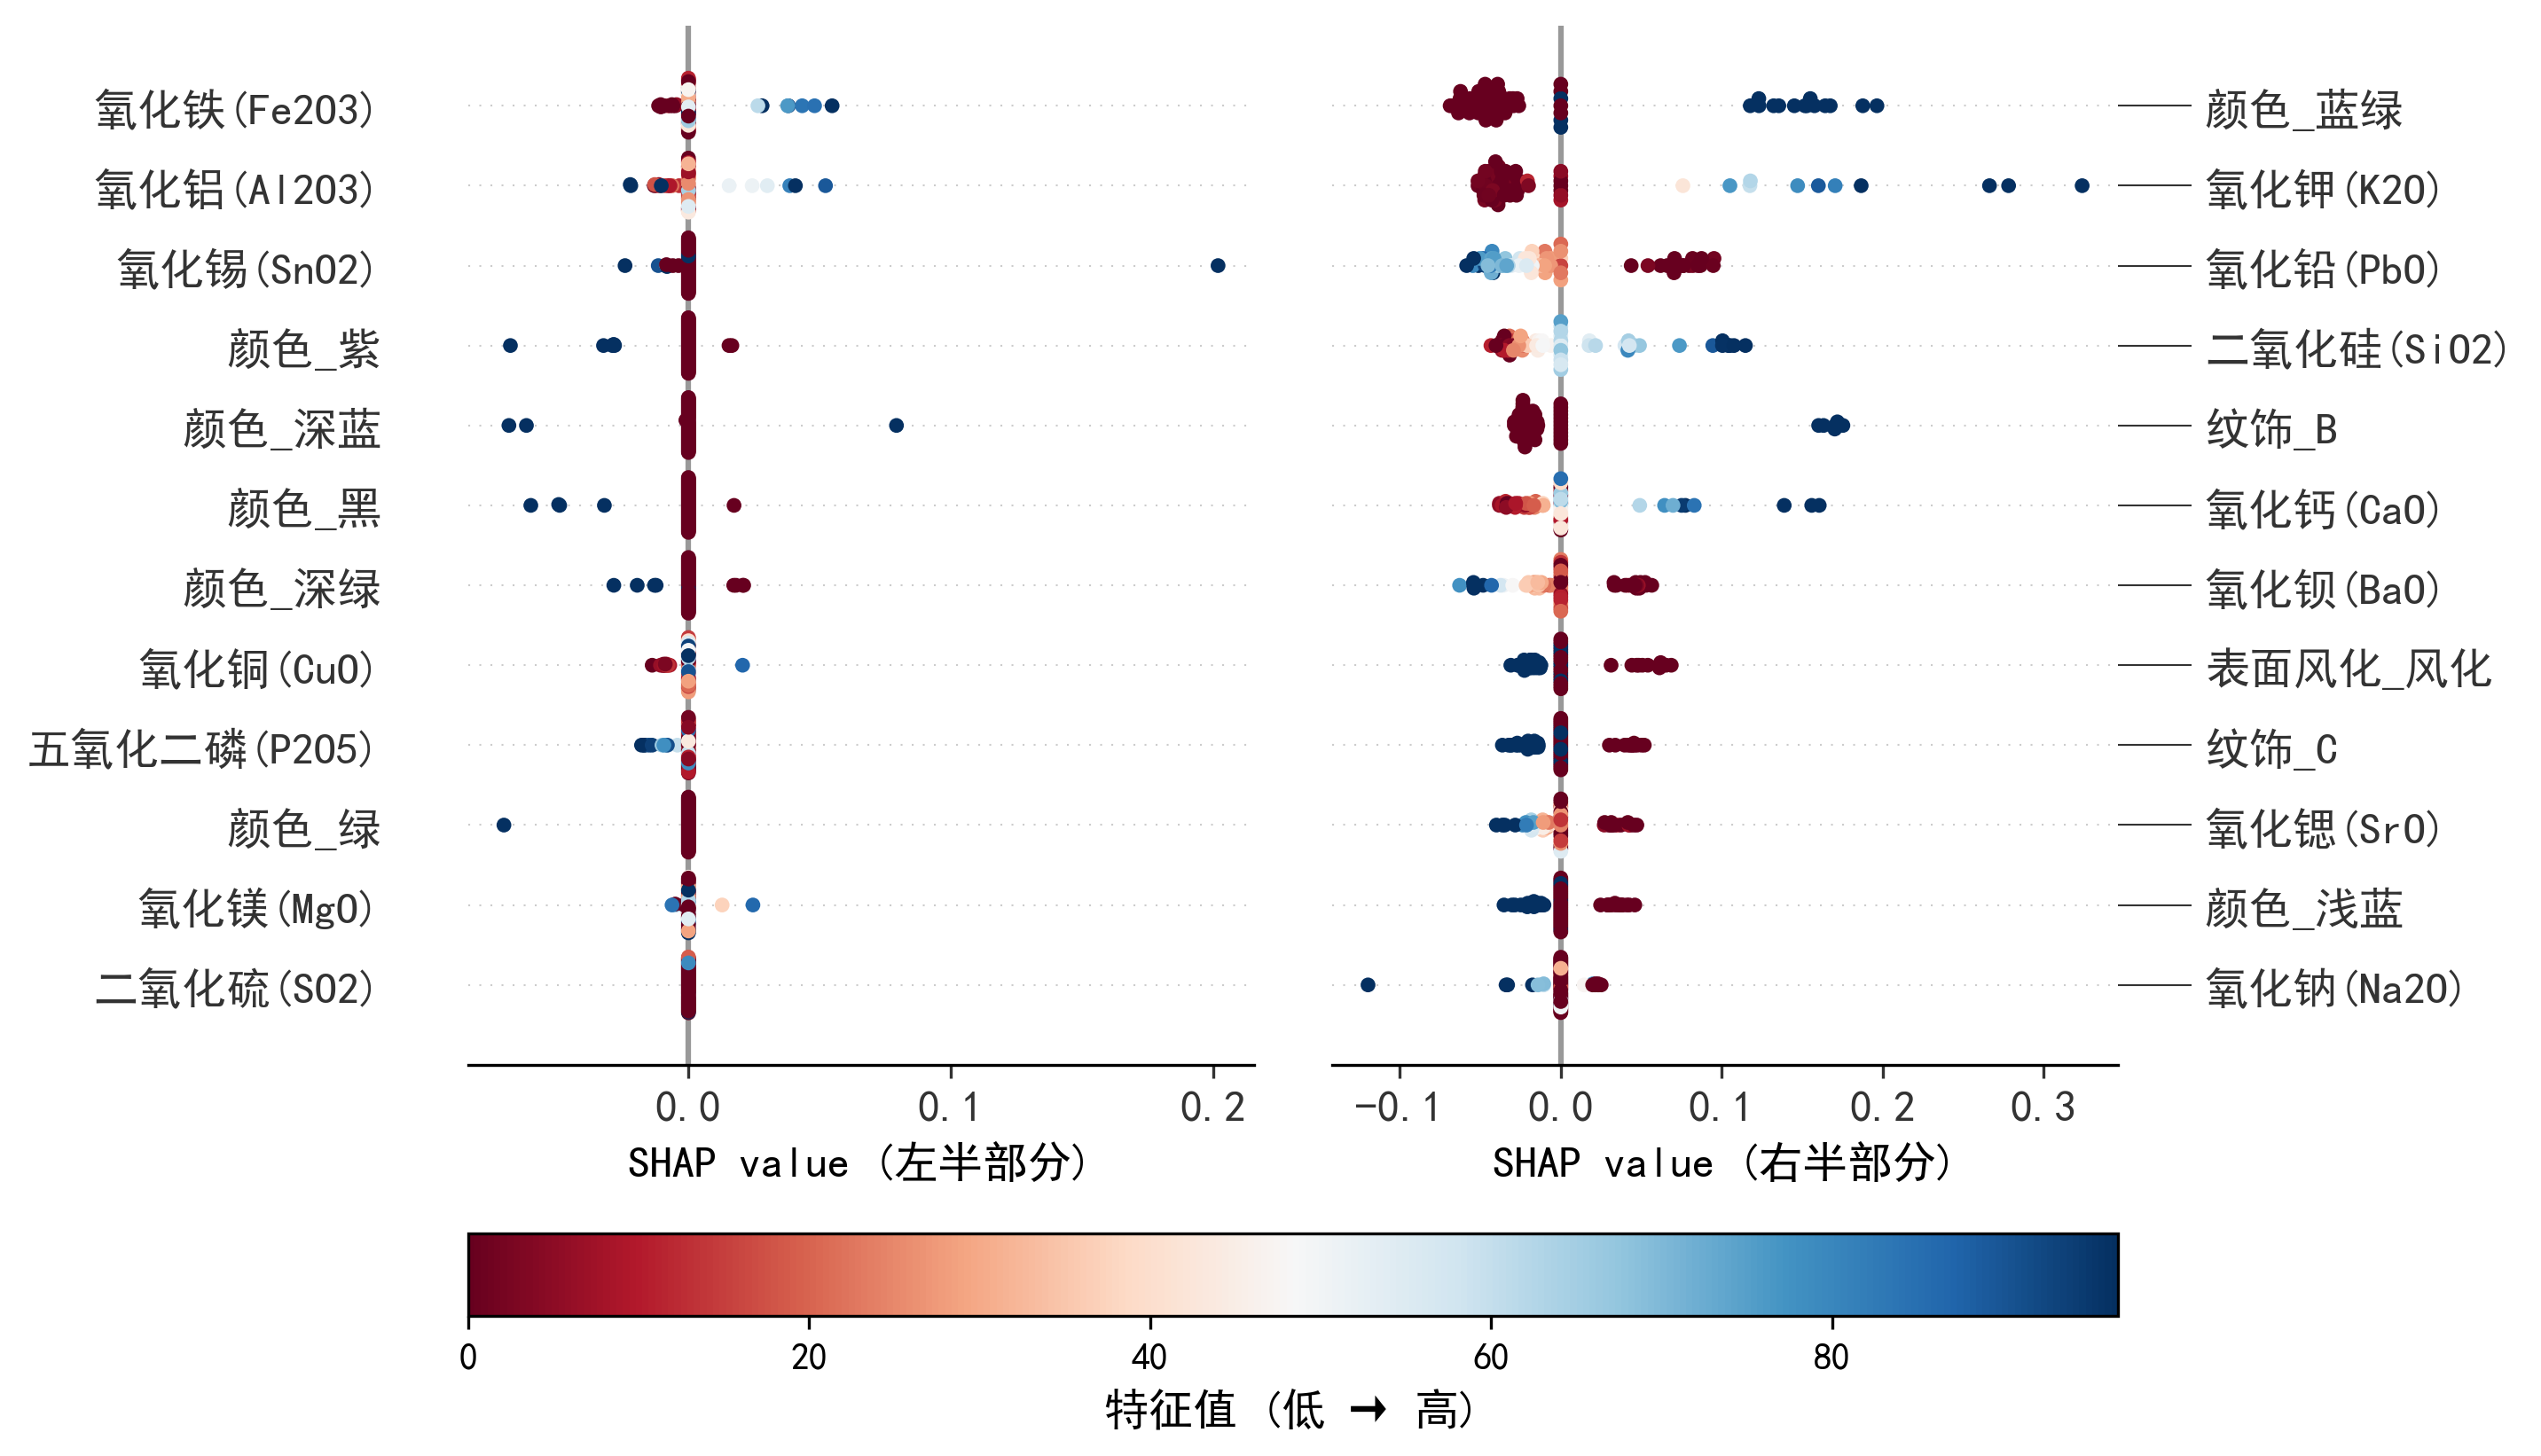
\includegraphics[width=\textwidth]{figs/4问题二/SHAP摘要图_双列_最终版_横置色条.png}
    \caption{非线性支持向量机模型的SHAP全局特征重要性分析}
    \label{fig:shap_summary}
\end{figure}

图\ref{fig:shap_summary}展示了全局特征重要性,纵轴按重要性高低排列特征,横轴是SHAP值,点的颜色代表该特征原始值的大小。该图再次确认$PbO$与$K_2O$是最重要的特征,并且提供了更丰富的细节,高含量的$PbO$红点总是对应着强烈的负向SHAP值,而高含量的$K_2O$红点则总是对应着强烈的正向SHAP值。

\subsection{各类别内部的亚类划分}

亚类划分的目标是探索同一类别文物之间是否存在基于化学成分的更细微群组。因此,分析的最小单元必须是文物个体,而非单个采样点。我们首先整合数据,对同一未风化文物的多个采样点取化学成分平均值,以消除采样位置带来的随机误差。对于风化文物,则优先选取能代表其风化状态的采样点数据进行平均。若风化文物缺乏此类数据,则采用分级条件均值插补,依据类型、颜色、纹饰的相似性为其估算一个风化后的化学成分。此过程最终生成了一个包含三十四个独立文物,且成分状态一致的数据集。

在进行聚类前,需要筛选出适合用于划分亚类的化学成分。亚类划分旨在寻找类别内部的差异,因此变异系数$CV$成为一个合适的指标。它是一个无量纲的相对离散度量,其定义如下
\begin{equation}
    CV = \frac{\sigma}{\mu}
\end{equation}
其中$\sigma$是标准差,$\mu$是均值。变异系数消除了不同化学成分自身含量均值大小的影响,能更公平地比较各特征的真实变异程度。我们据此为高钾和铅钡玻璃分别筛选出类内变异程度最高的化学成分作为聚类特征。
为确定各类玻璃内部可能存在的亚类数量,我们首先采用探索性的层次聚类方法。该方法无需预设类别数量,通过计算样本间的距离,将化学成分最相似的样本逐级合并,其过程可以通过树状图进行可视化。

\begin{figure}[H]
    \centering
    \begin{minipage}{0.48\textwidth}
        \centering
        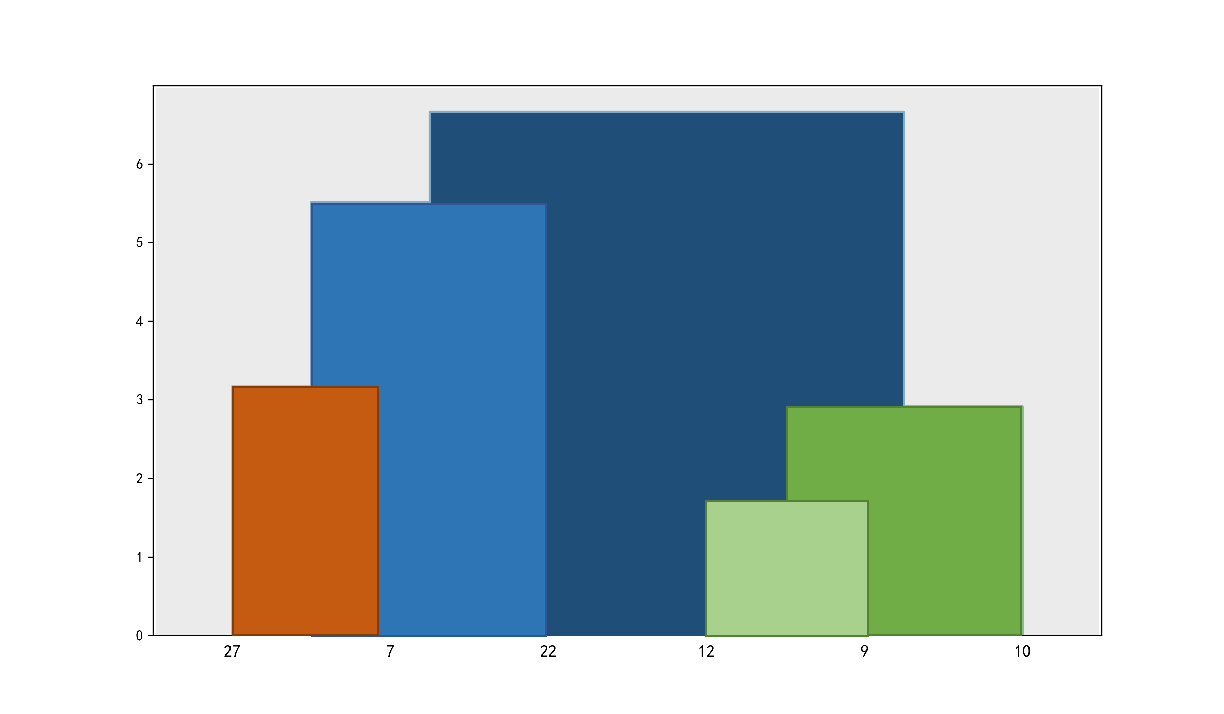
\includegraphics[width=\linewidth]{figs/4问题二/高钾玻璃_层次聚类树状图.png}
        \caption{高钾玻璃层次聚类树状图}
        \label{fig:hclust_k}
    \end{minipage}\hfill
    \begin{minipage}{0.48\textwidth}
        \centering
        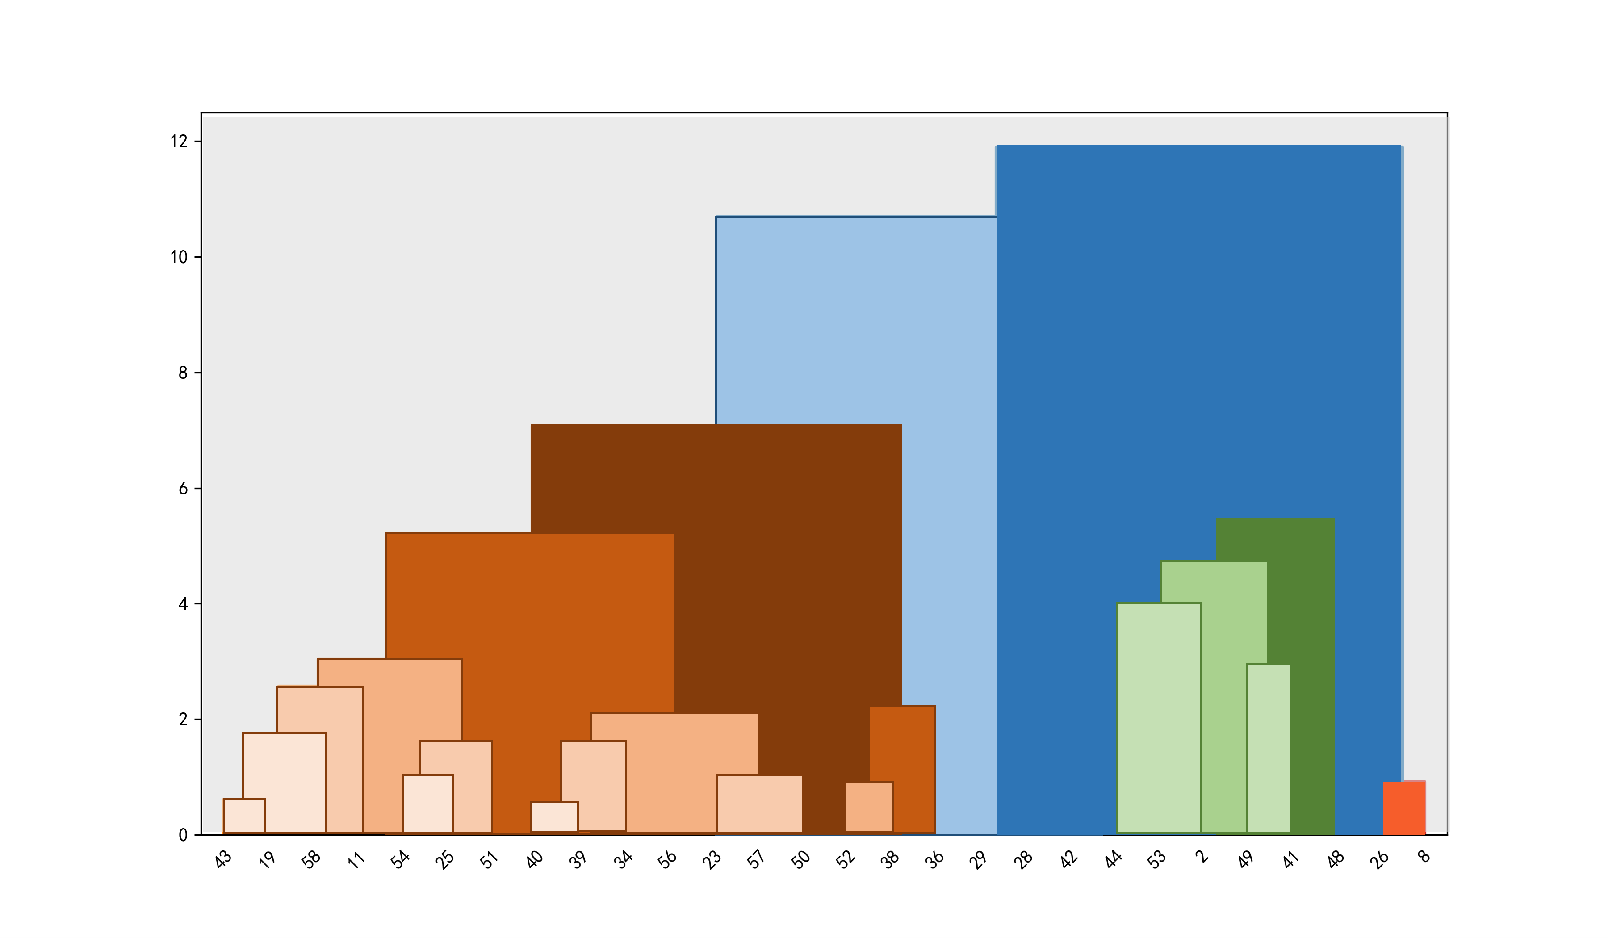
\includegraphics[width=\linewidth]{figs/4问题二/铅钡玻璃_层次聚类树状图.png}
        \caption{铅钡玻璃层次聚类树状图}
        \label{fig:hclust_pb}
    \end{minipage}
\end{figure}

图\ref{fig:hclust_pb}展示的铅钡玻璃树状图呈现出清晰的两分支结构,两个主分支在较高的距离水平上才发生合并,这初步表明铅钡玻璃样本可自然地分为两个大类。相比之下,图\ref{fig:hclust_k}中高钾玻璃的树状图结构更为复杂,呈现出多层次的嵌套聚合模式,表示其内部可能存在更多数量的亚类。

为对亚类数量的选择提供定量依据,我们引入轮廓系数指标。该指标综合评估每个样本与其所属簇的相似度即内聚性,以及与其他簇的差异度即分离度。轮廓系数值越接近一,表示聚类结果的结构越合理。

\begin{figure}[H]
    \centering
    \begin{minipage}{0.48\textwidth}
        \centering
        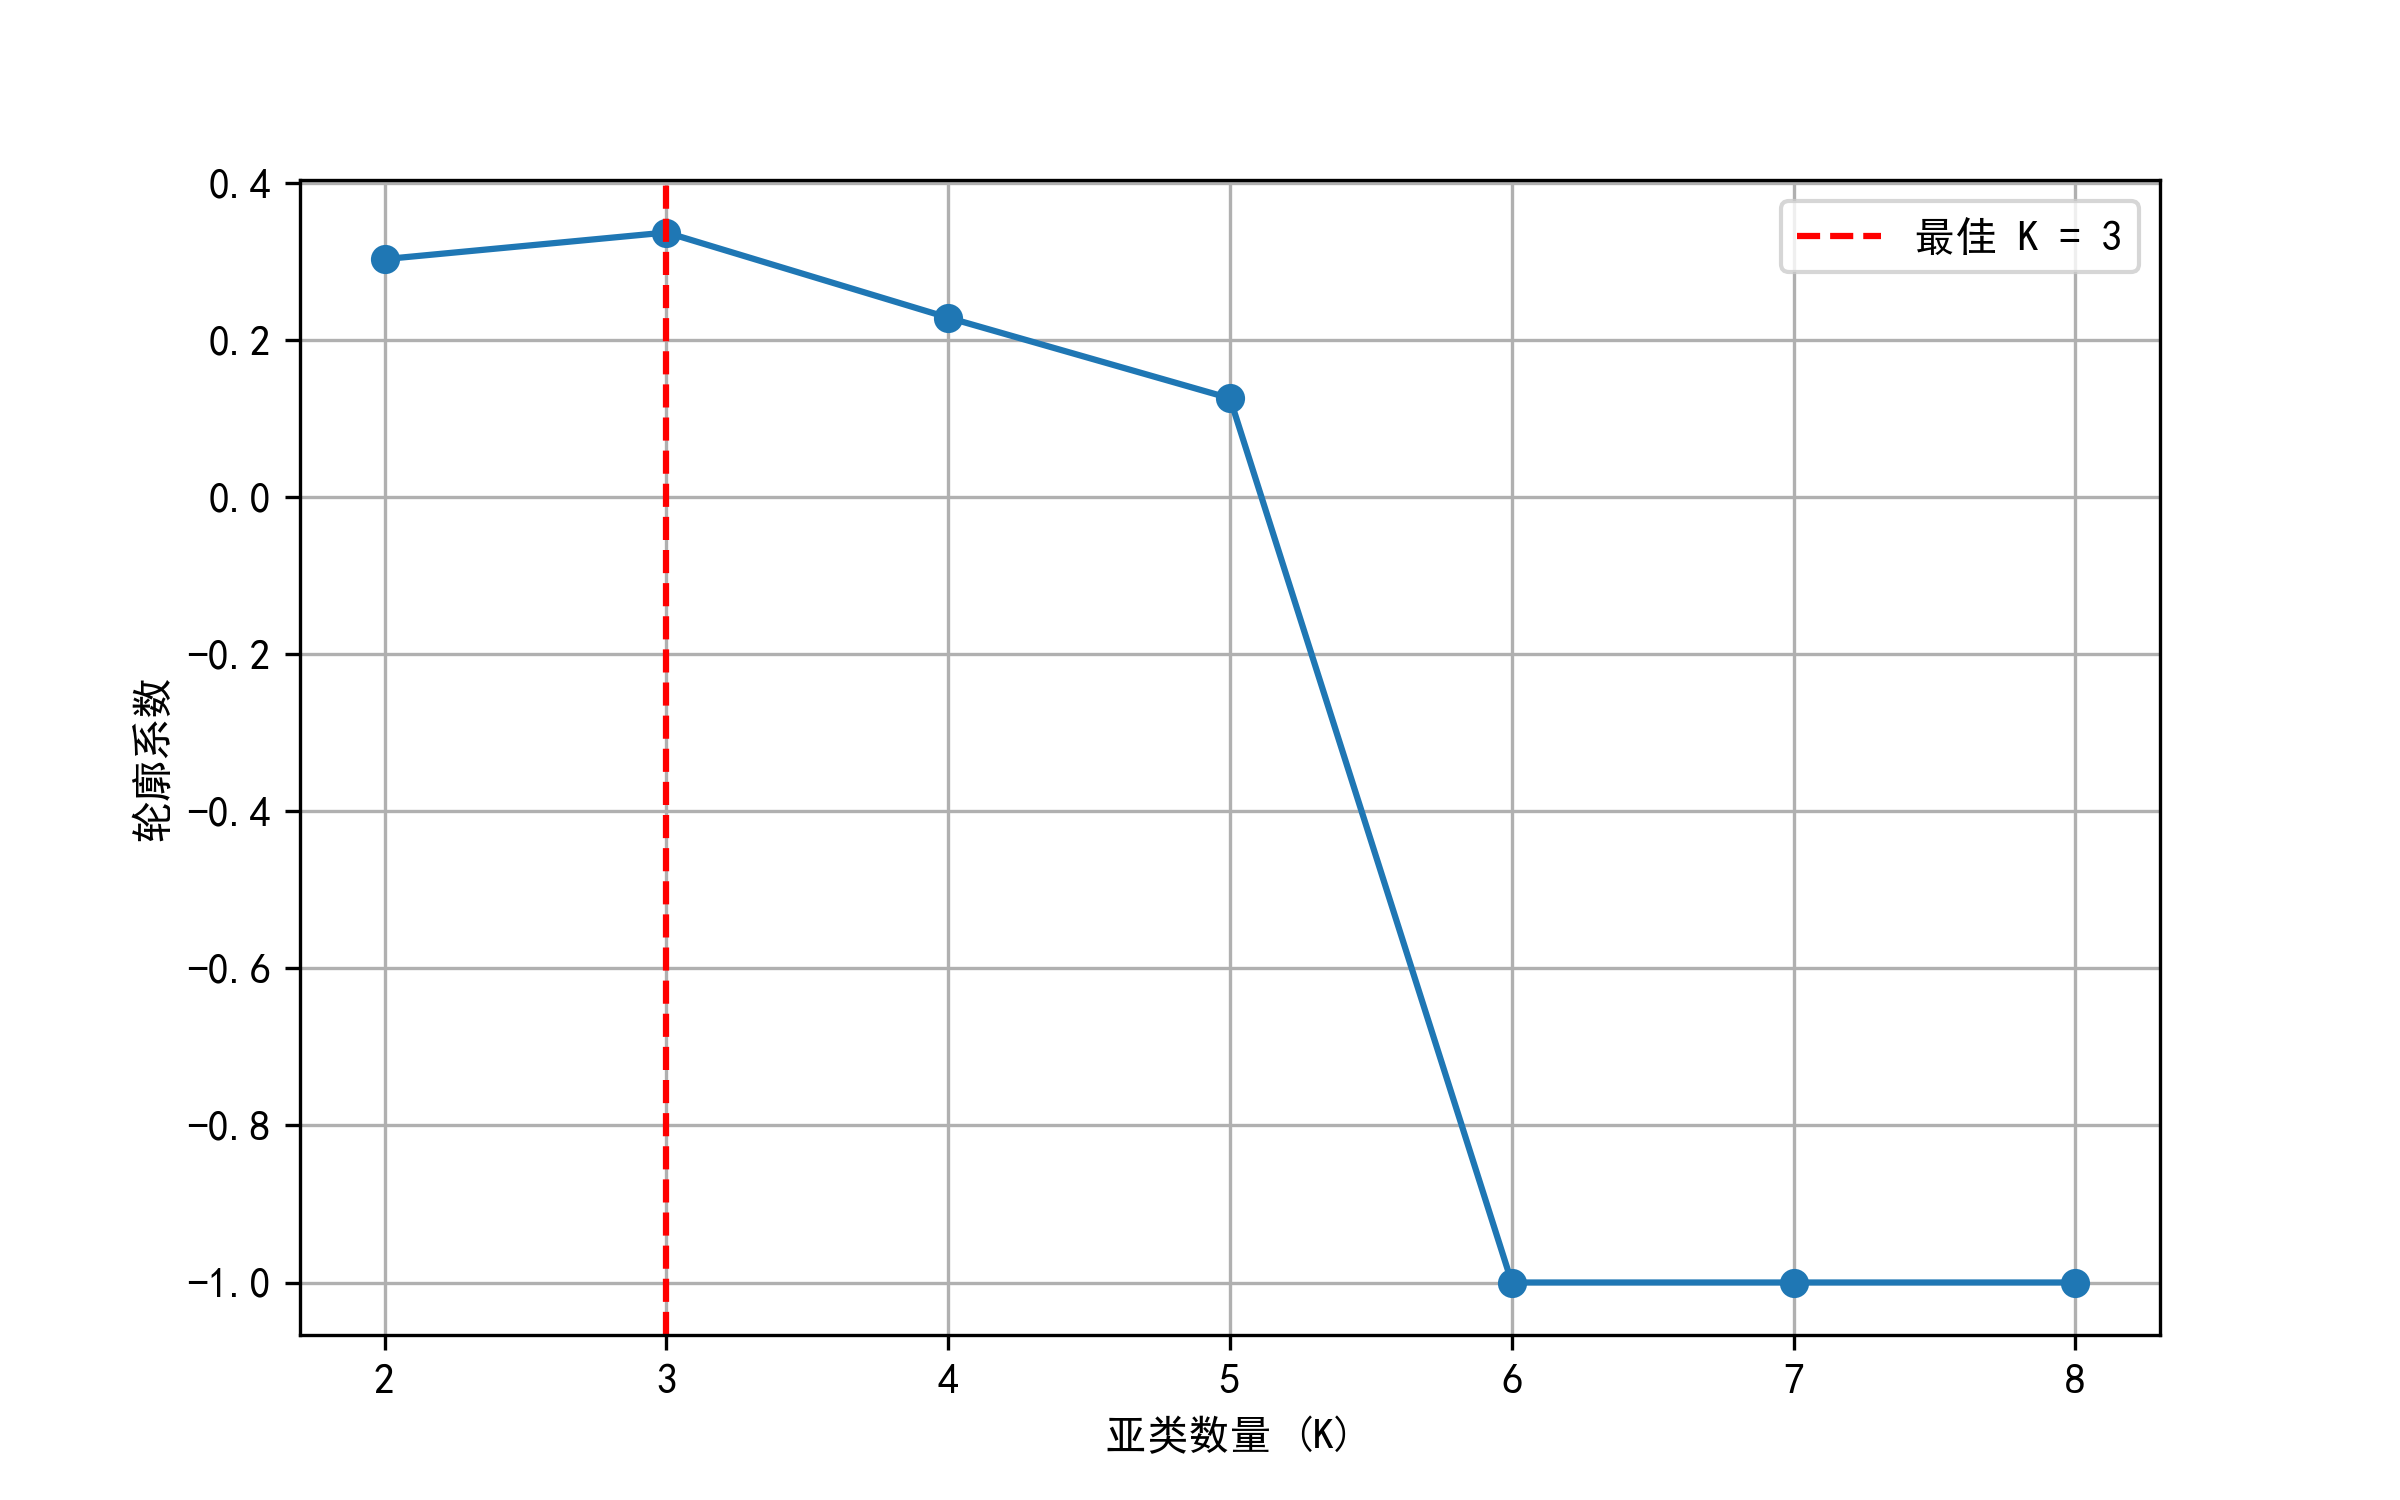
\includegraphics[width=\linewidth]{figs/4问题二/高钾玻璃_最佳K值选择.png}
        \caption{高钾玻璃轮廓系数随K值的变化}
        \label{fig:k_select_k}
    \end{minipage}\hfill
    \begin{minipage}{0.48\textwidth}
        \centering
        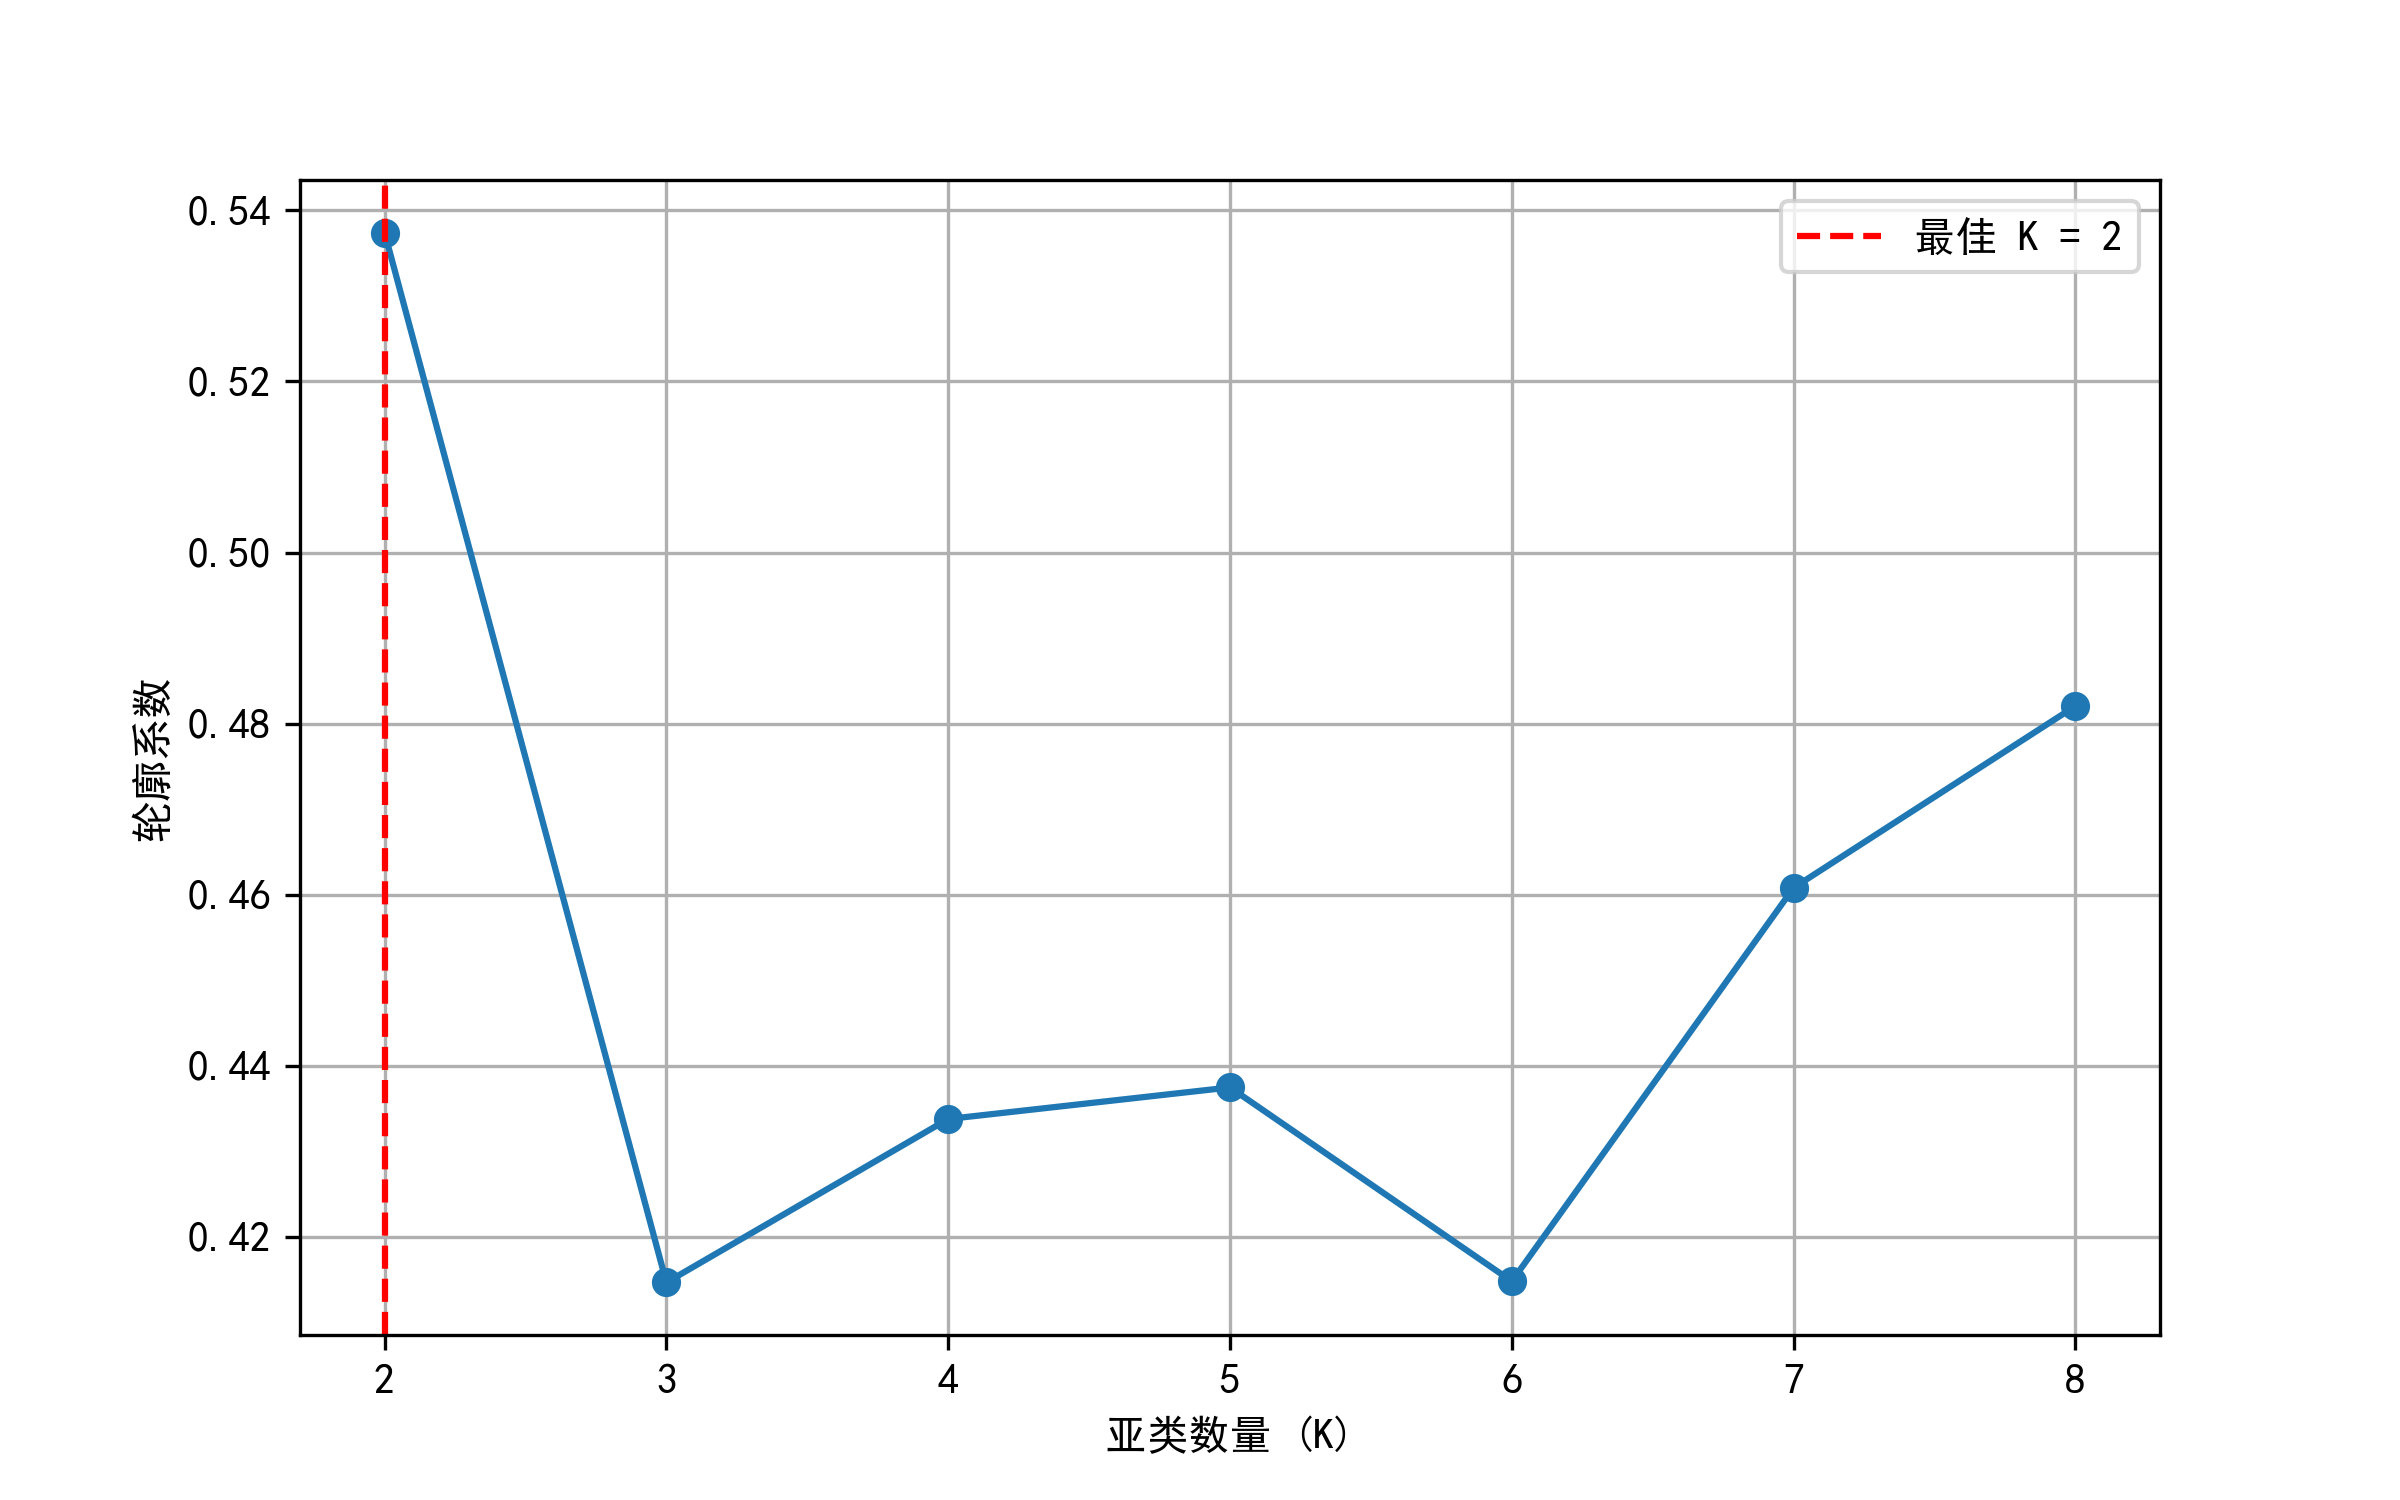
\includegraphics[width=\linewidth]{figs/4问题二/铅钡玻璃_最佳K值选择.png}
        \caption{铅钡玻璃轮廓系数随K值的变化}
        \label{fig:k_select_pb}
    \end{minipage}
\end{figure}

如图\ref{fig:k_select_pb}所示,对于铅钡玻璃,轮廓系数在$K=2$时取得最大值,约为零点四八,当$K$值继续增加时,系数值出现明显下降。对于高钾玻璃,如图\ref{fig:k_select_k}所示,轮廓系数在$K=5$时达到峰值,约为零点五二。综合定性观察与定量计算,我们将铅钡玻璃的亚类数量确定为二,高钾玻璃的亚类数量确定为五。

为验证划分结果的有效性并解读各亚类的化学特征,我们首先利用主成分分析方法将高维的化学成分数据投影到二维平面上。

\begin{figure}[H]
    \centering
    \begin{minipage}{0.48\textwidth}
        \centering
        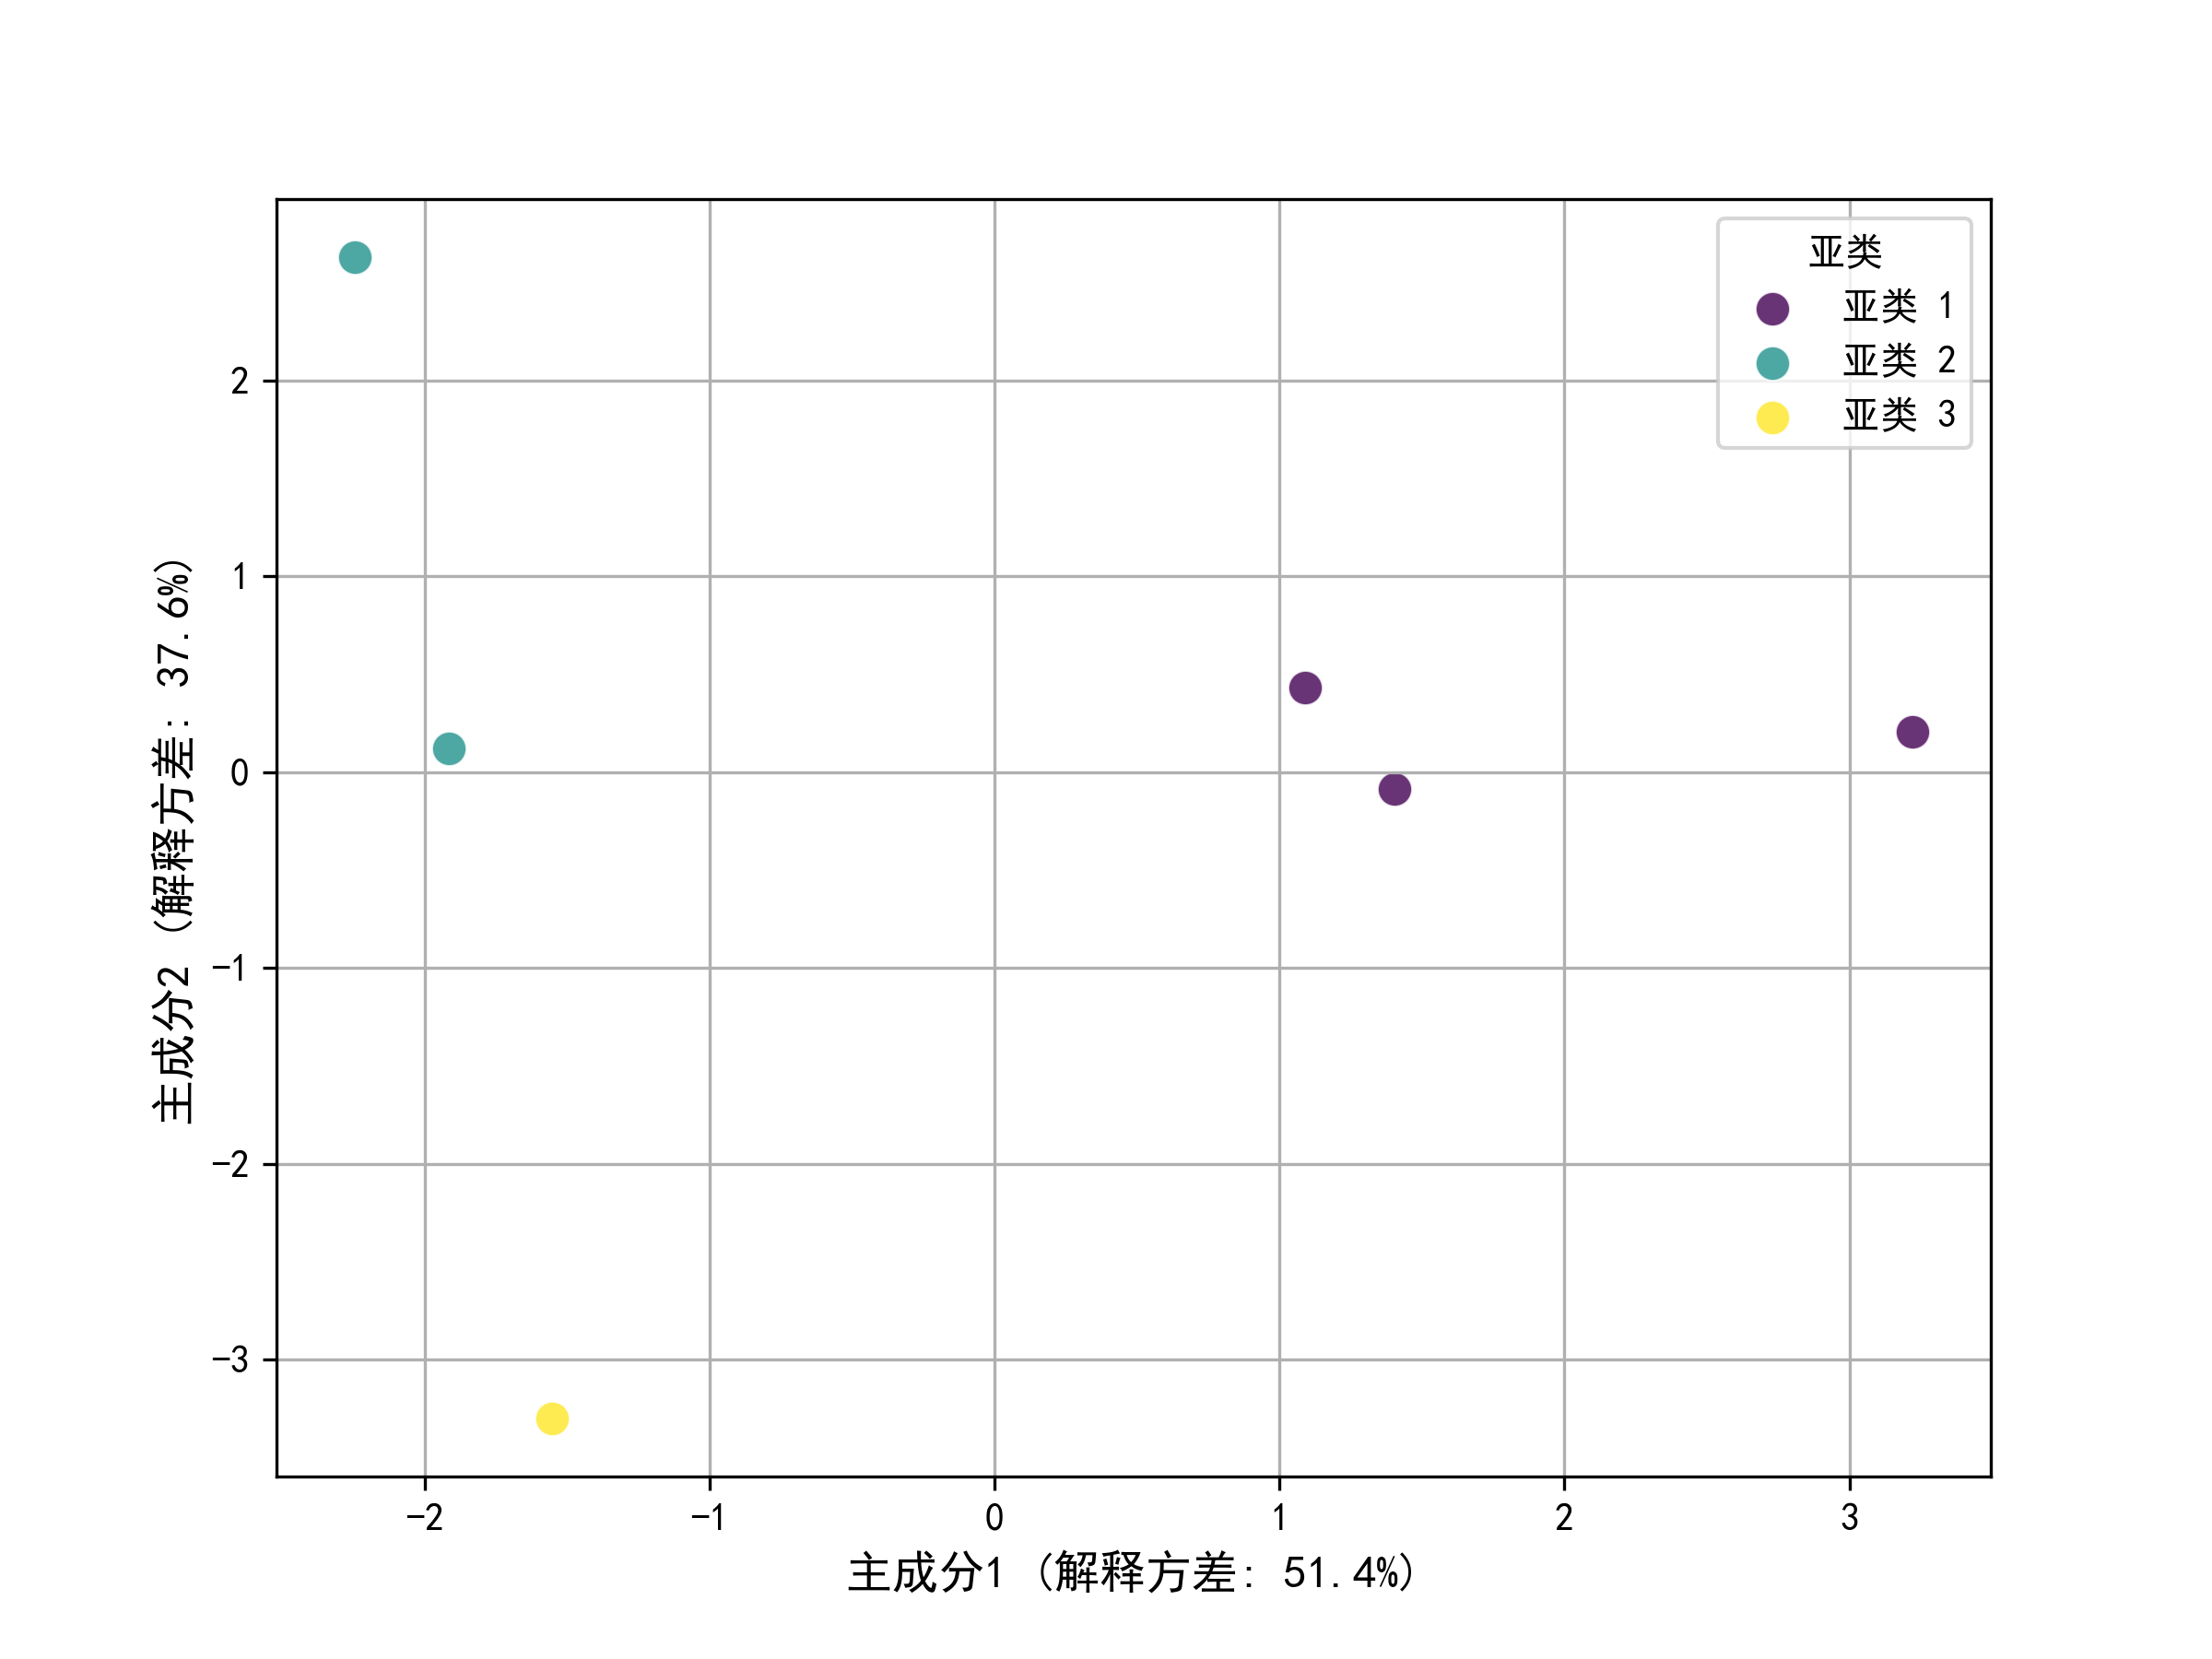
\includegraphics[width=\linewidth]{figs/4问题二/高钾玻璃_亚类PCA图.png}
        \caption{高钾玻璃亚类划分PCA可视化}
        \label{fig:pca_k}
    \end{minipage}\hfill
    \begin{minipage}{0.48\textwidth}
        \centering
        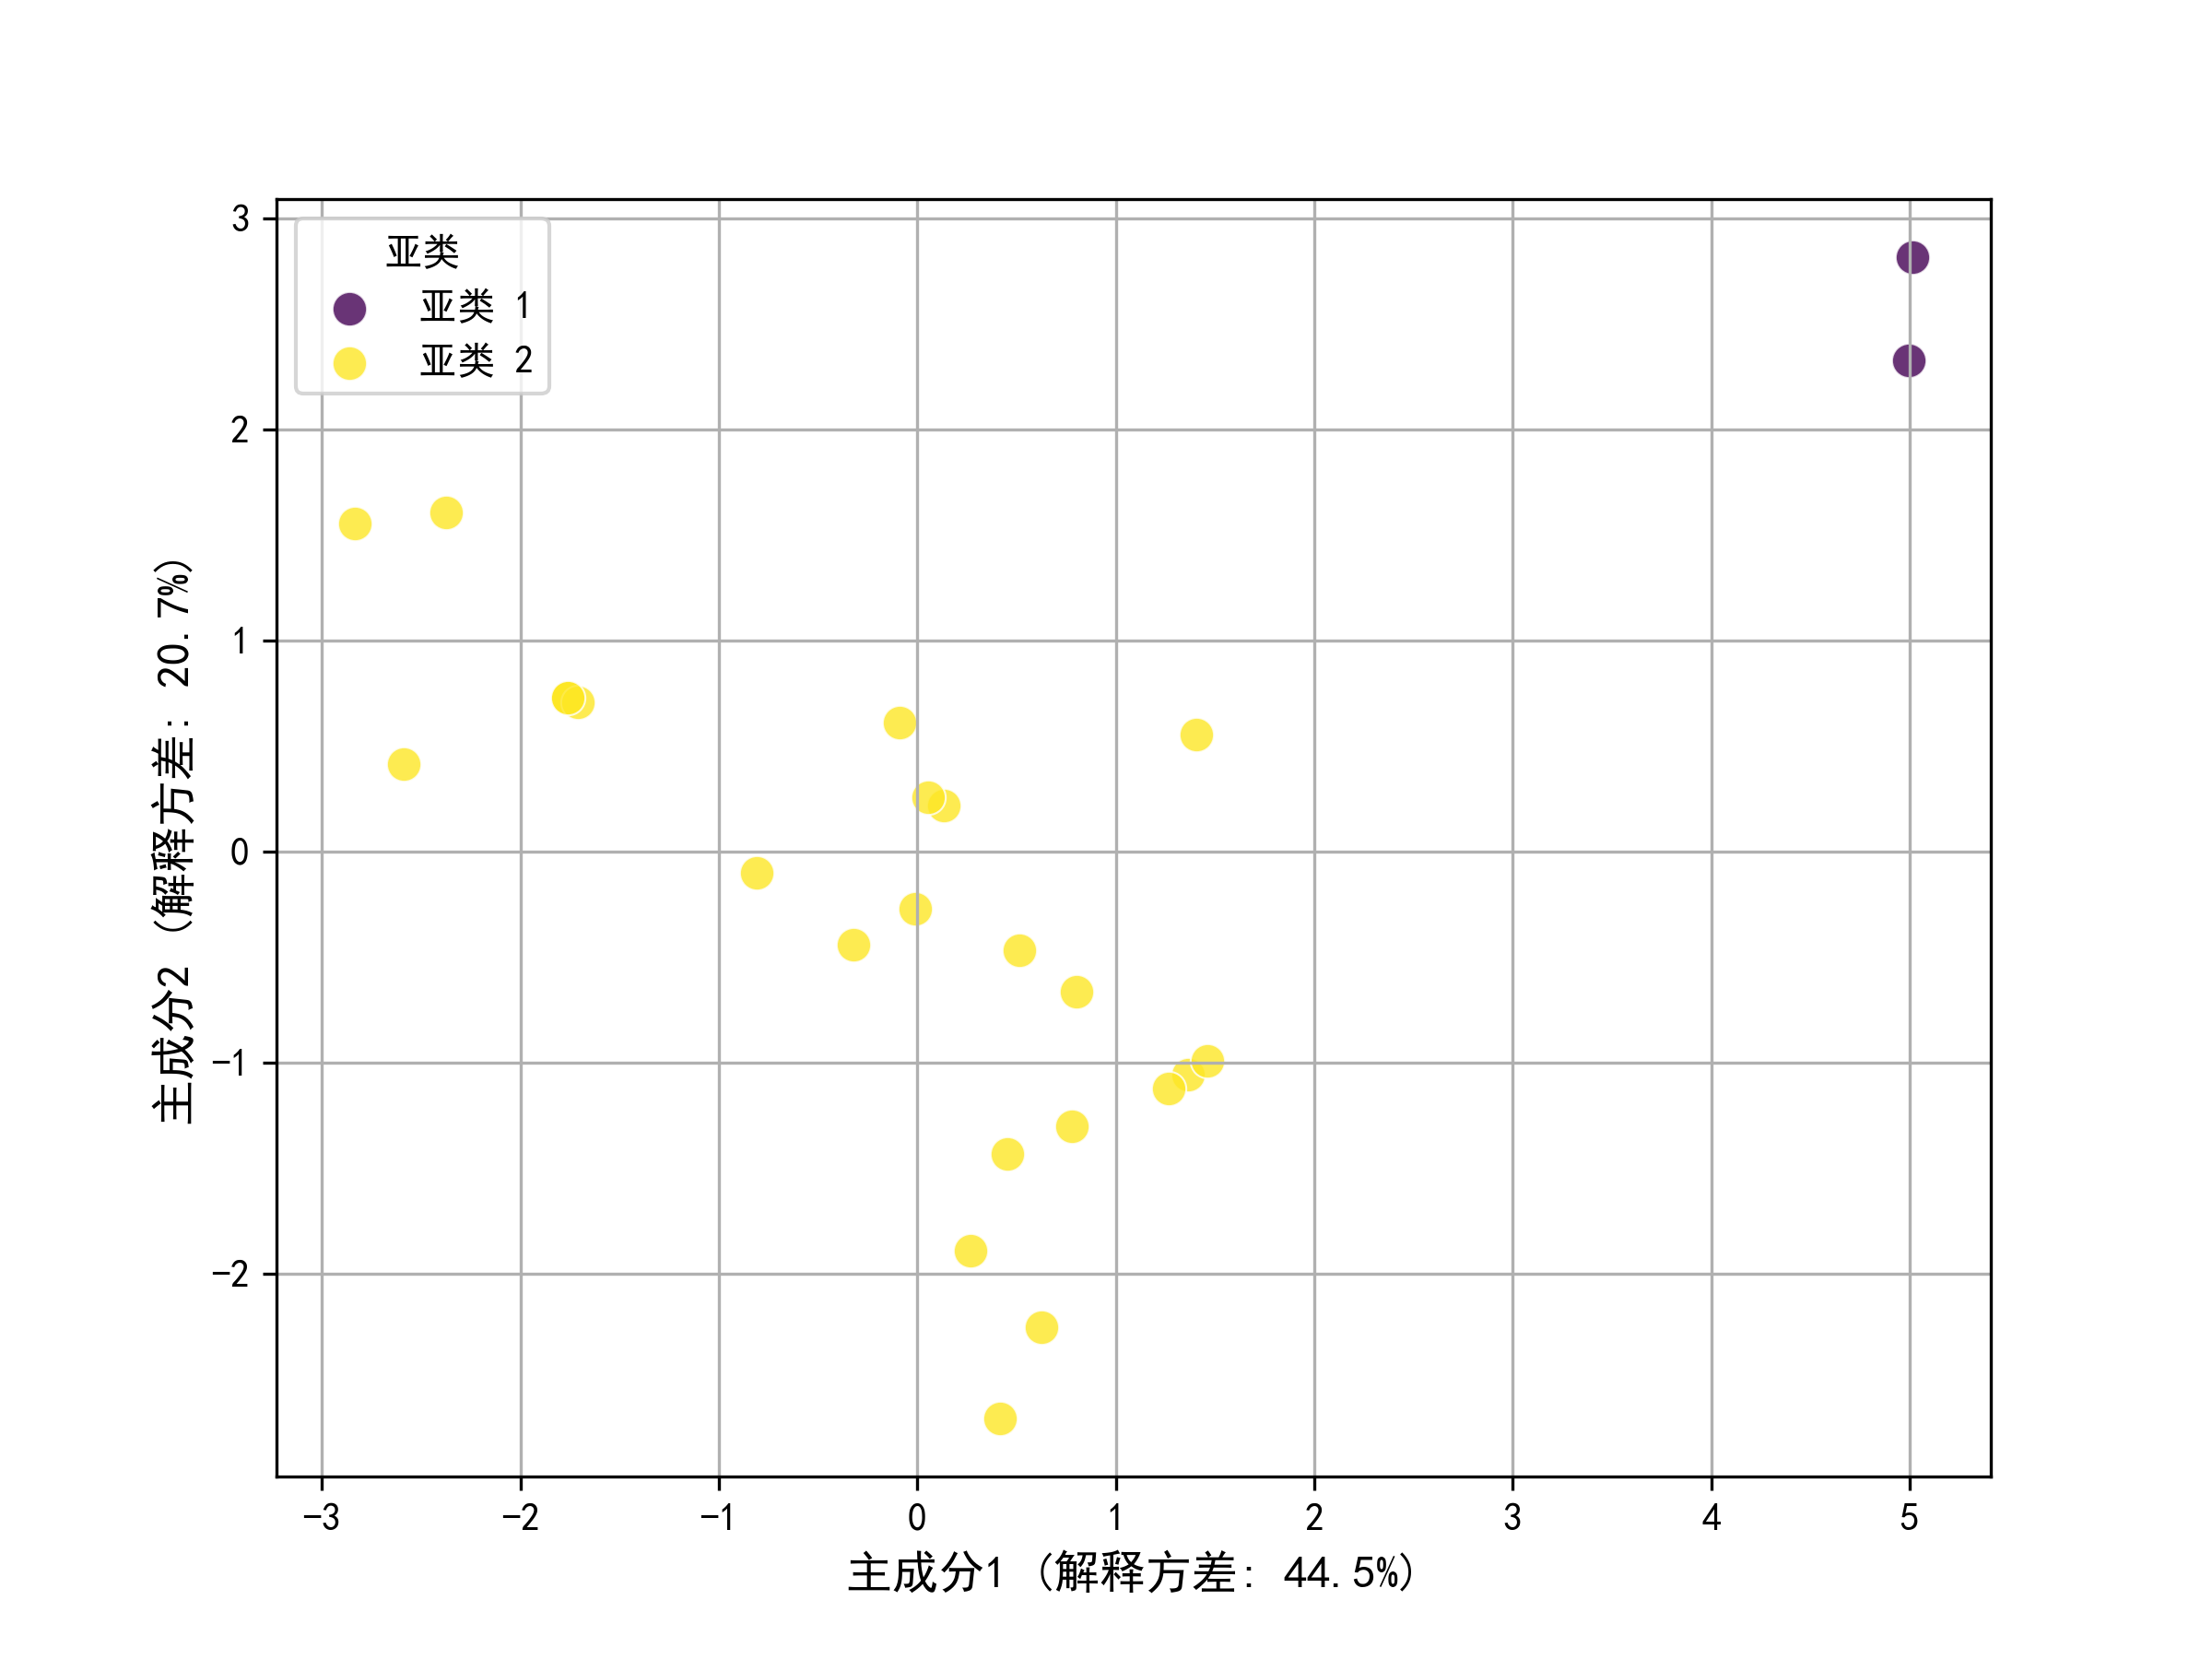
\includegraphics[width=\linewidth]{figs/4问题二/铅钡玻璃_亚类PCA图.png}
        \caption{铅钡玻璃亚类划分PCA可视化}
        \label{fig:pca_pb}
    \end{minipage}
\end{figure}

图\ref{fig:pca_k}与图\ref{fig:pca_pb}的可视化结果显示,不同颜色的点代表不同亚类的样本。铅钡玻璃的两个亚类在第一主成分轴上具有显著的分离。高钾玻璃的五个亚类也在二维空间中占据了相对独立的区域,各亚类内部样本较为集中,而亚类之间存在明显界限。

为进一步阐释每个亚类所代表的化学成分模式,我们绘制了亚类化学特征热力图。

\begin{figure}[H]
    \centering
    \begin{minipage}{0.48\textwidth}
        \centering
        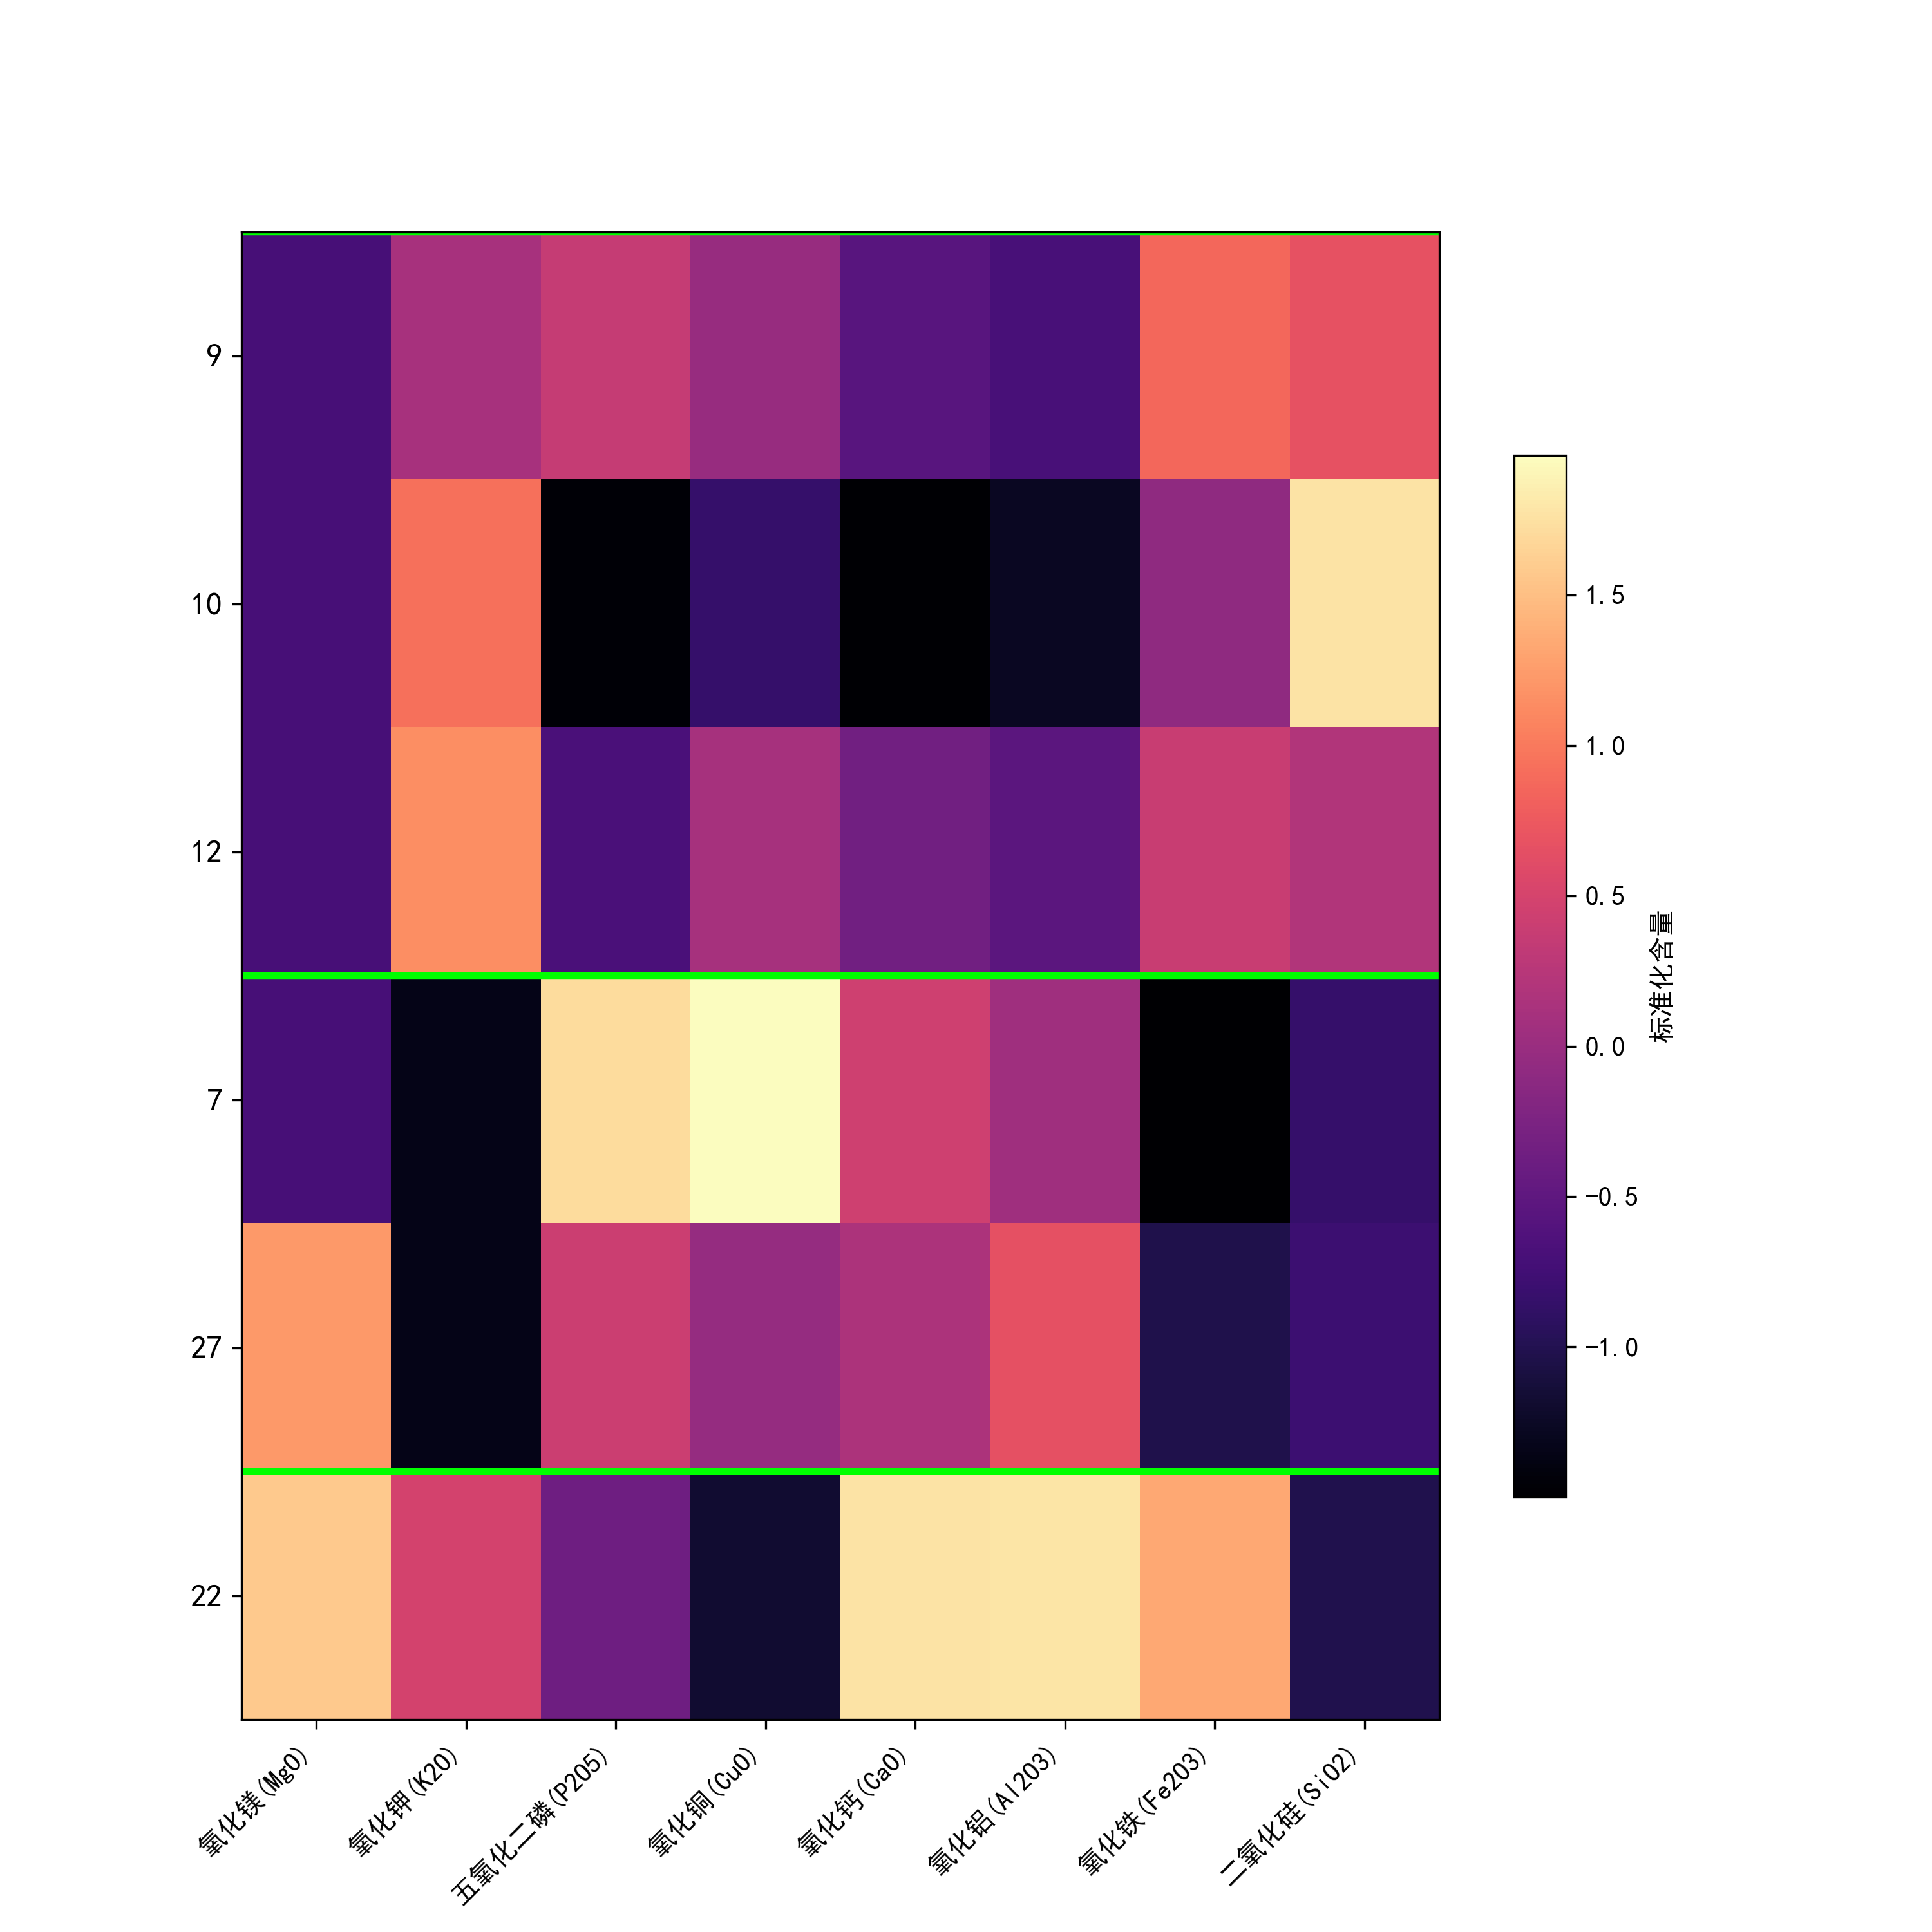
\includegraphics[width=\linewidth]{figs/4问题二/高钾玻璃_亚类热力图_带编号.png}
        \caption{高钾玻璃亚类化学特征热力图}
        \label{fig:heatmap_k}
    \end{minipage}\hfill
    \begin{minipage}{0.48\textwidth}
        \centering
        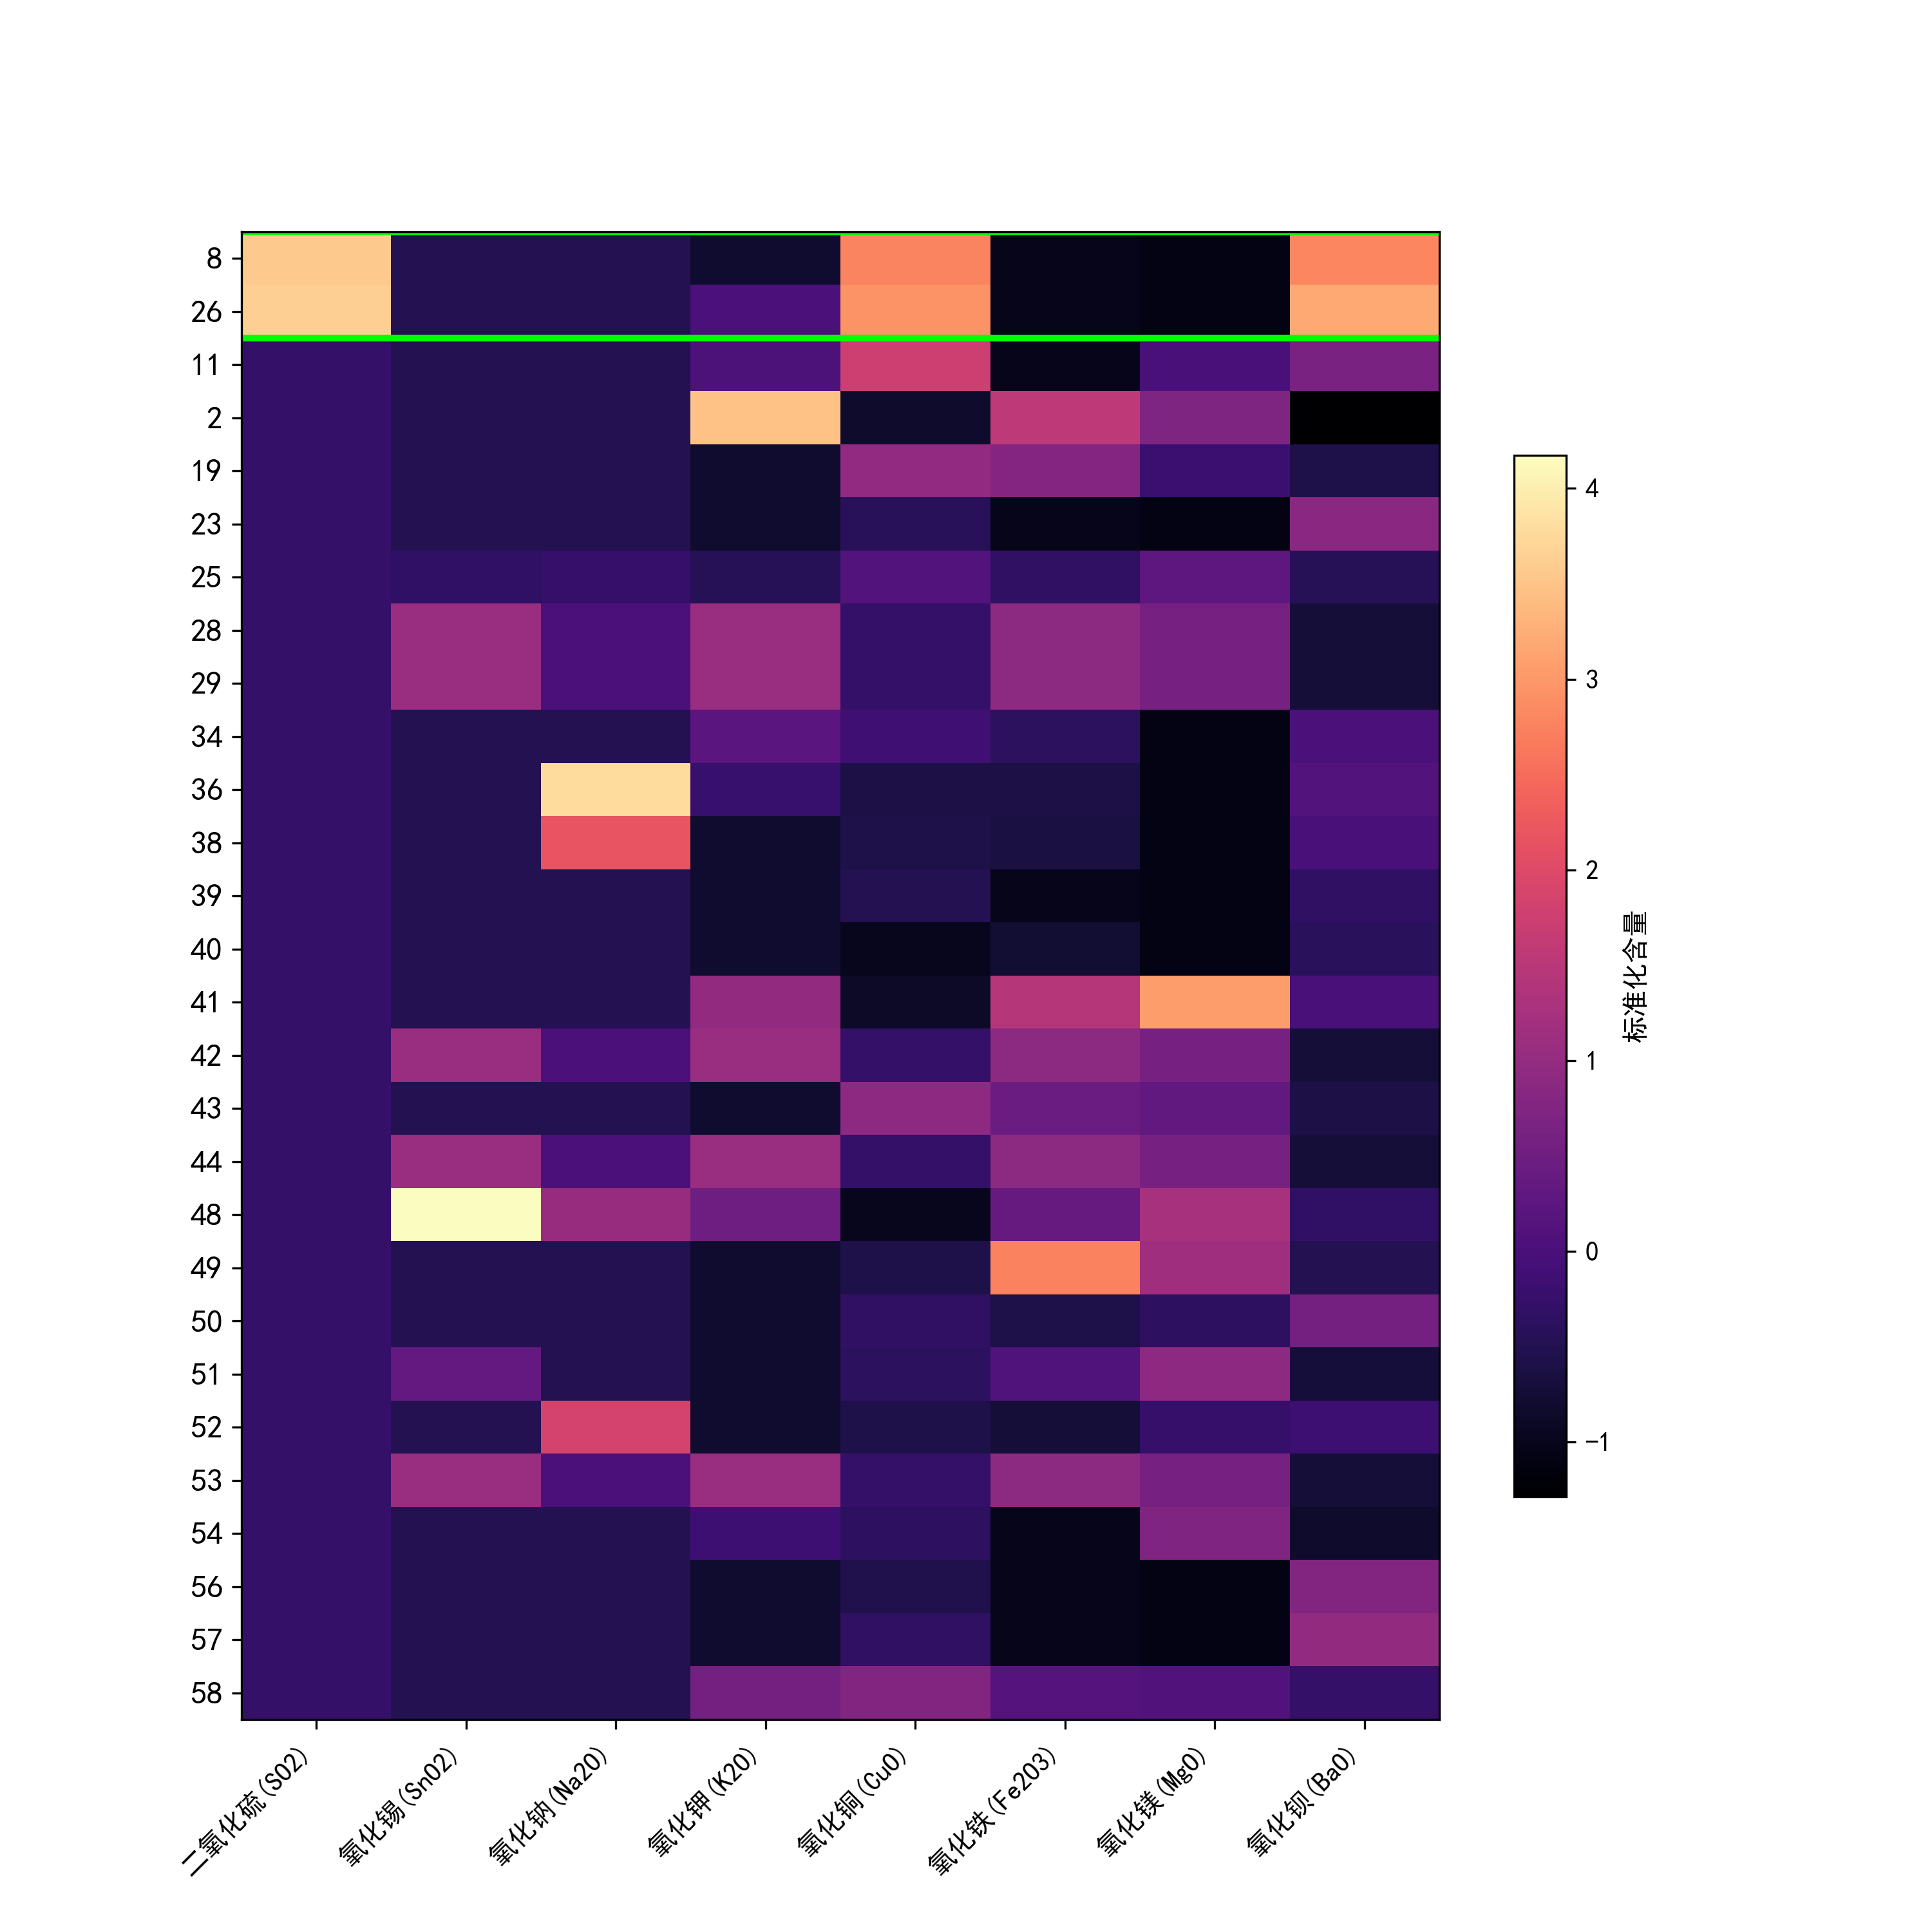
\includegraphics[width=\linewidth]{figs/4问题二/铅钡玻璃_亚类热力图_带编号.png}
        \caption{铅钡玻璃亚类化学特征热力图}
        \label{fig:heatmap_pb}
    \end{minipage}
\end{figure}

图\ref{fig:heatmap_pb}展示了铅钡玻璃两个亚类的化学差异。亚类一的样本在氧化铅$PbO$与氧化钡$BaO$两种助熔剂成分上呈现深色,表明其含量普遍较高,而作为玻璃基体的二氧化硅$SiO_2$含量则相对较低。与此相反,亚类零的样本在二氧化硅$SiO_2$上呈现深色,含量普遍较高,而氧化铅$PbO$与氧化钡$BaO$含量则较低。基于此,可将亚类一命名为高铅钡助熔剂型,亚类零命名为高硅基质型。

图\ref{fig:heatmap_k}则展现了高钾玻璃五个亚类更为细微的化学特征。亚类二的突出特征是其氧化钾$K_2O$含量极高,而其他成分含量较低。亚类一的氧化钙$CaO$含量相对突出。亚类零则表现为氧化铝$Al_2O_3$与氧化铁$Fe_2O_3$含量较高,这可能与其他亚类使用了不同的矿物原料有关。亚类三与亚类四的差异主要体现在磷与硫等微量元素上,反映了更为精细的原料或工艺差别。通过热力图分析,我们明确了每个亚类独特的化学成分特征。


\subsection{结果的敏感性分析}

为验证上述分类与划分结果的稳健性,我们进行了敏感性分析。首先,我们检验分类规律的可靠性。我们在十折交叉验证的每一次折叠中,重新训练线性支持向量机模型并提取其权重,以评估规律本身的稳定性。

\begin{figure}[H]
    \centering
    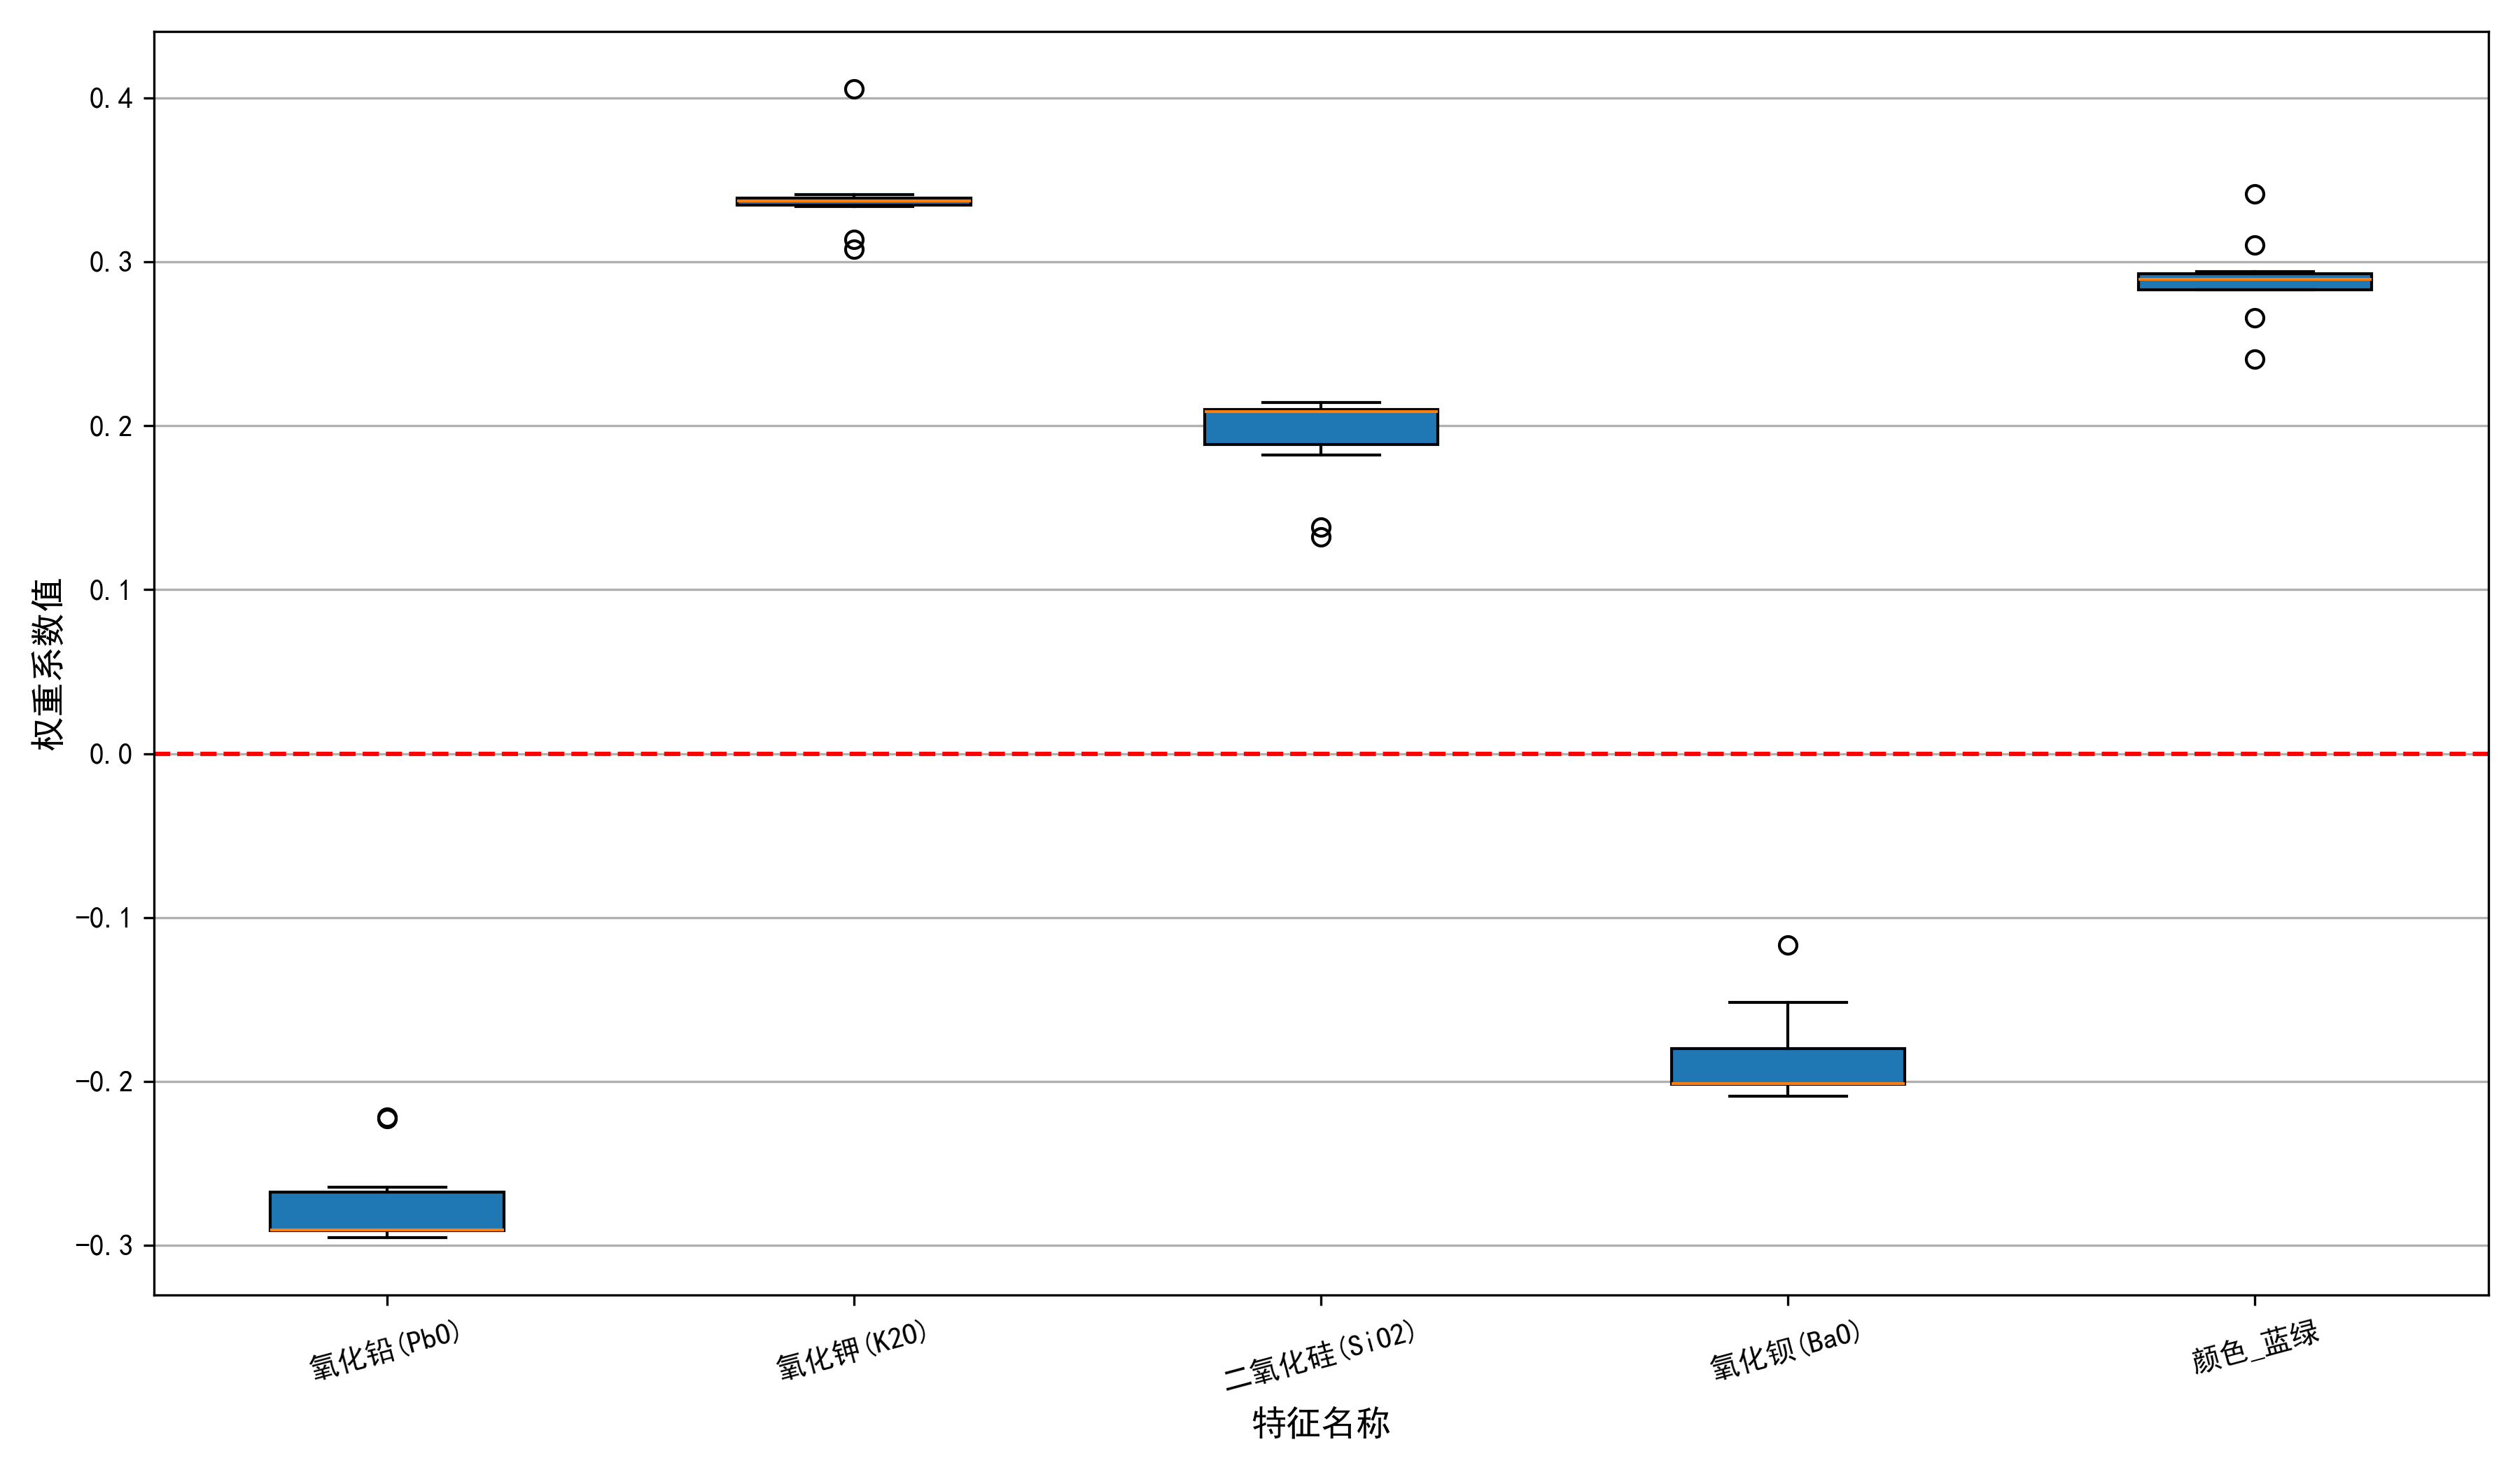
\includegraphics[width=\textwidth]{figs/4问题二/SVM权重稳定性分析.png}
    \caption{关键特征的SVM权重在十次交叉验证中的稳定性}
    \label{fig:svm_stability}
\end{figure}

图\ref{fig:svm_stability}通过箱线图展示了关键特征的权重在十次不同数据子集训练中的分布。图中显示,关键特征如$PbO$、$K_2O$的权重符号在十次实验中从未改变,且波动范围很小。这证明了我们提炼出的分类规律是高度稳健的。

其次,我们检验亚类划分结果的敏感性。为检验划分结果对化学成分测量误差的容忍度,我们采用了特征值扰动法。该方法通过向数据中注入不同水平的随机噪声,来模拟测量误差,并检验聚类结构的稳定性。我们对筛选出的特征数据乘以一个范围在$[1-p, 1+p]$内的随机扰动因子,其中$p$为扰动水平。在此扰动数据上重新聚类,并使用调整兰德指数$ARI$来衡量该次聚类结果与原始基准结果的一致性。

\begin{figure}[H]
    \centering
    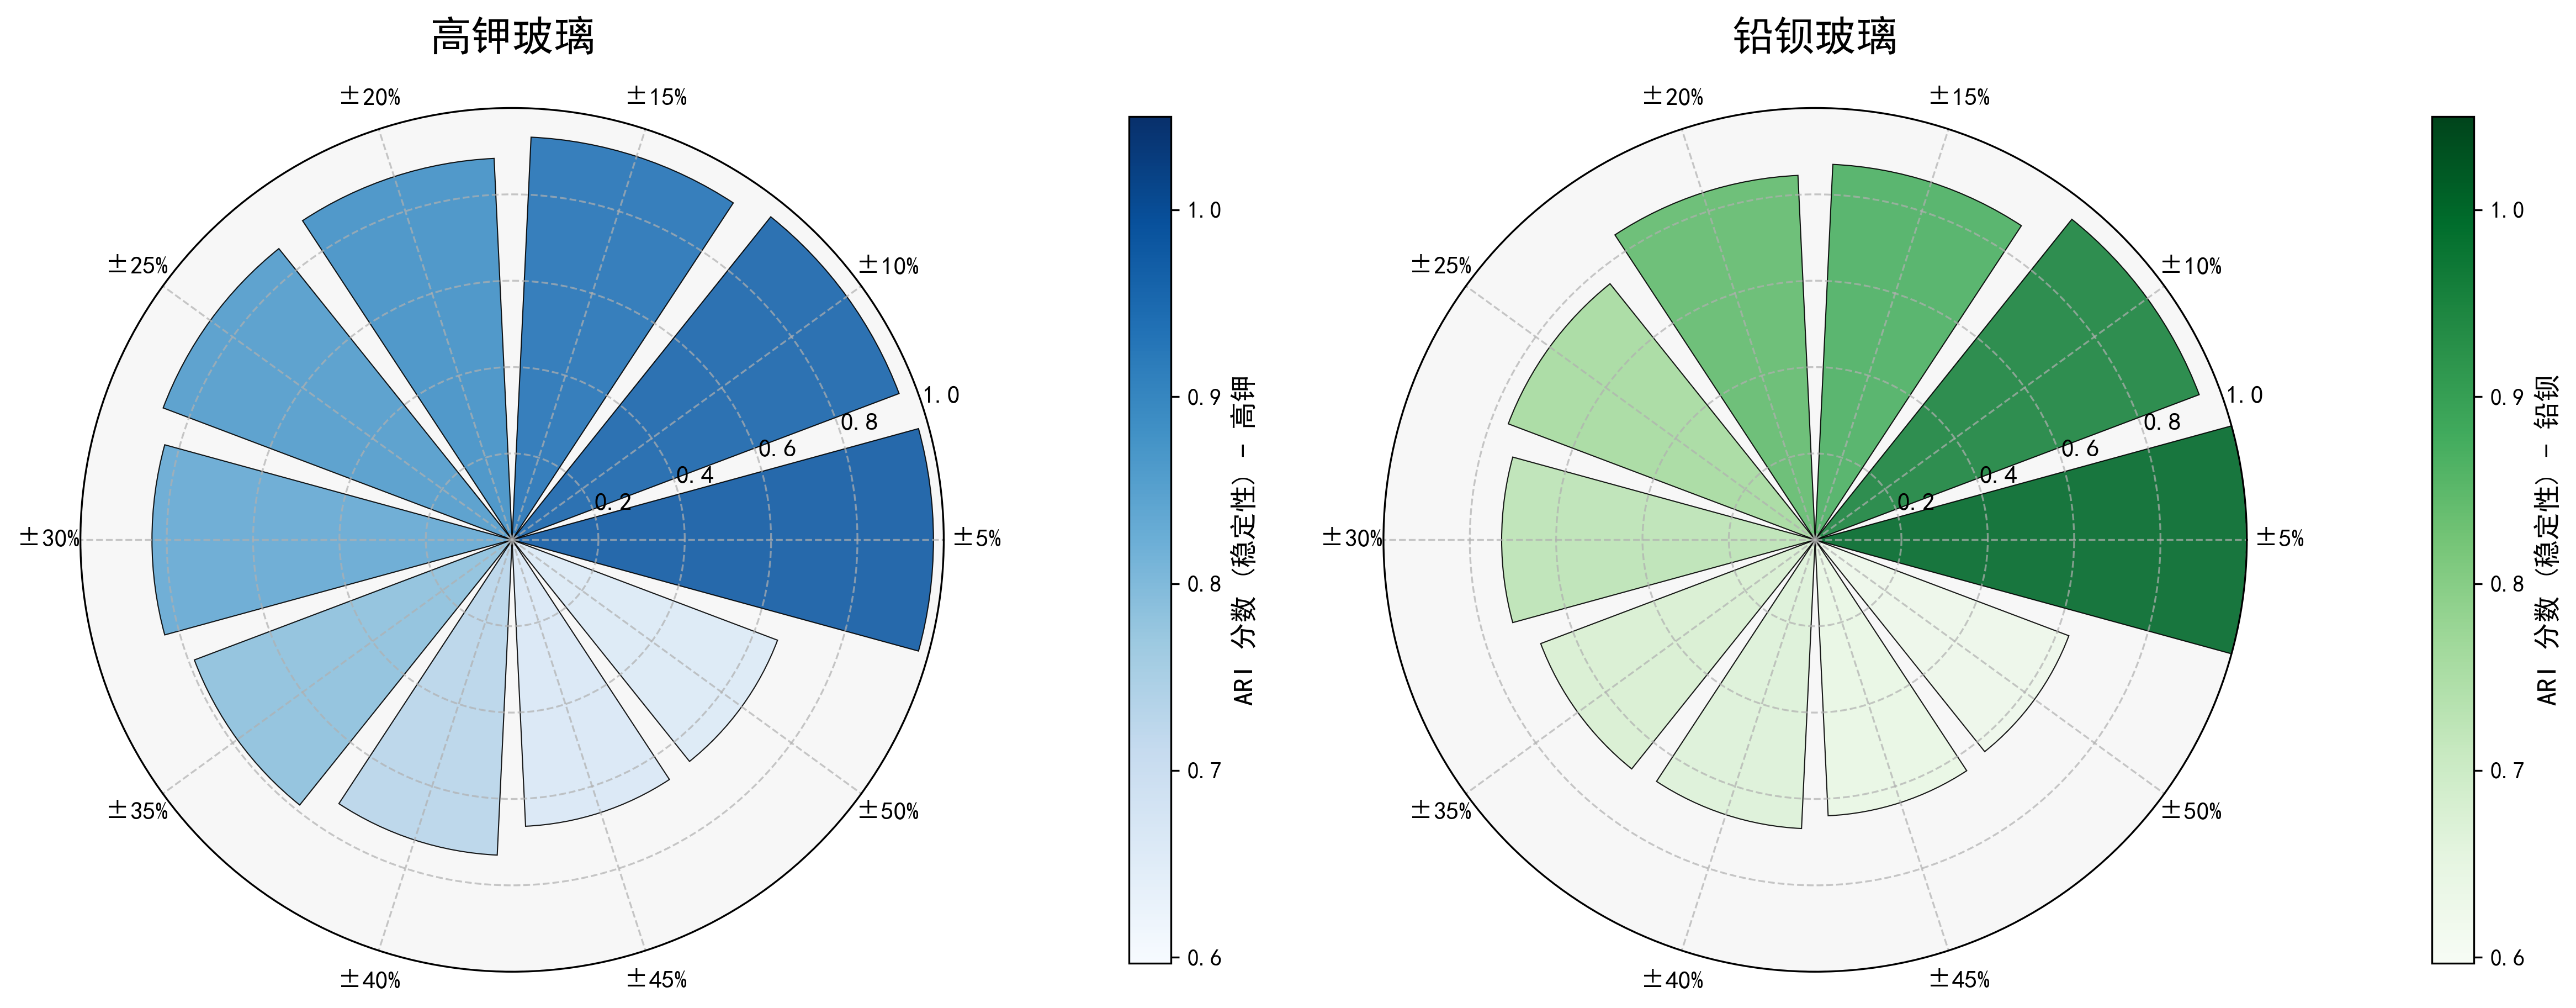
\includegraphics[width=\textwidth]{figs/4问题二/灵敏度分析_玫瑰图_ARI颜色映射.png}
    \caption{不同扰动水平下亚类划分结果的ARI分数}
    \label{fig:ari_sensitivity}
\end{figure}

图\ref{fig:ari_sensitivity}展示了在不同扰动水平下,高钾和铅钡玻璃亚类划分的平均ARI分数。对于高钾玻璃,即使在百分之十的扰动下,平均ARI分数依然高达0.9513。对于铅钡玻璃,在百分之十的扰动下,平均ARI分数为0.9596。在面临潜在的测量误差时,其核心划分依然能够保持高度一致。这证明了我们发现的亚类结构是真实且稳健的,而非随机产生的现象。


